% Art der Arbeit: Bachelorarbeit
% Titel: "BLAST Avionics Thermal Management"
% Autor: Viktor Hoffmann
%-----------------------------------------------------------------------------------
% verwendete Packages
\documentclass{ITLR}
% Use ITLR.cls for first style-definition. 
% IMPORTANT: change in ITLR.cls colors in hyperref-package ONLY for printing; NOT for PDF submittance


% ----------- Zusätzliche Usepackages ----------------------------------------------
% Hier stehen weitere Usepackages ...
\usepackage{siunitx}
\usepackage{tikz}
\usepackage{subcaption}
\usetikzlibrary{arrows.meta}
\usepackage{acronym}
\usepackage{pdfpages}
\usepackage{booktabs}
\usepackage{listings}
\usepackage{xcolor}
\usepackage{float} % für [H]-Option
\usepackage{makecell}

\lstset{
  basicstyle=\ttfamily\small,
  keywordstyle=\color{blue},
  stringstyle=\color{green!60!black},
  commentstyle=\color{gray},
  numbers=left,
  numberstyle=\tiny,
  frame=single,
  breaklines=true,
  captionpos=b
}

% ----------- Graphics Paths -------------------------------------------------------
\graphicspath{{Bilder/}}

%###################################################################################
% ----------- Dokumentanfang -------------------------------------------------------
\begin{document}
\setstretch{1.1667} 		% Zeilenabstand (Verhältnis, hier z.B. 14pt/12pt)
\pagestyle{Abstract}		% oben definiert

% ----------- Title & Preface  -----------------------------------------------------
\pagenumbering{Alph}
%\begin{titlepage}
%---- ITLR-Logo ----
\begin{figure}[ht]
     \centering
      
\includegraphics[width=65mm]{./Logos/ITLR_Logo.eps}
\end{figure}

\hspace{200mm}

%---- Title of the study thesis ----
\begin{center}
    \begin{Large}
        Bachelorarbeit
    \end{Large}

    \vspace{2.5mm}

    \BRule
    \vspace{2.5mm}
    \begin{LARGE}
    \\
        Entwicklung des Avionik-Thermal-Managements einer Experimentalrakete
        \\
    \vspace{1mm}
    \end{LARGE}
    \vspace{2.5mm}
    \BRule
    \vspace{15mm}

    \begin{Large}

    Viktor Hoffmann \\
    
\end{Large}

\end{center}

\vfill

%---- Uni-Logo ----
\begin{wrapfigure}[4]{l}{17mm}
    
\includegraphics[width=17mm]{./Logos/unilogo_neu}
\end{wrapfigure}

\parbox[t]{120mm}
{
    \sffamily
      \vspace{3mm}
        Universität~Stuttgart\\
        \textbf{Institut~für~Thermodynamik~der~Luft-~und~Raumfahrt~(ITLR)}\\[2mm]
        Direktor: Prof.~Dr.-Ing.~habil.~Bernhard~Weigand
}




\end{titlepage}


\includepdf{Text/Hoffmann_BA_Deckblatt2.pdf}
\newpage\null\thispagestyle{empty}\newpage

\includepdf{Text/Aufgabenstellung_BA_Hoffmann.pdf}
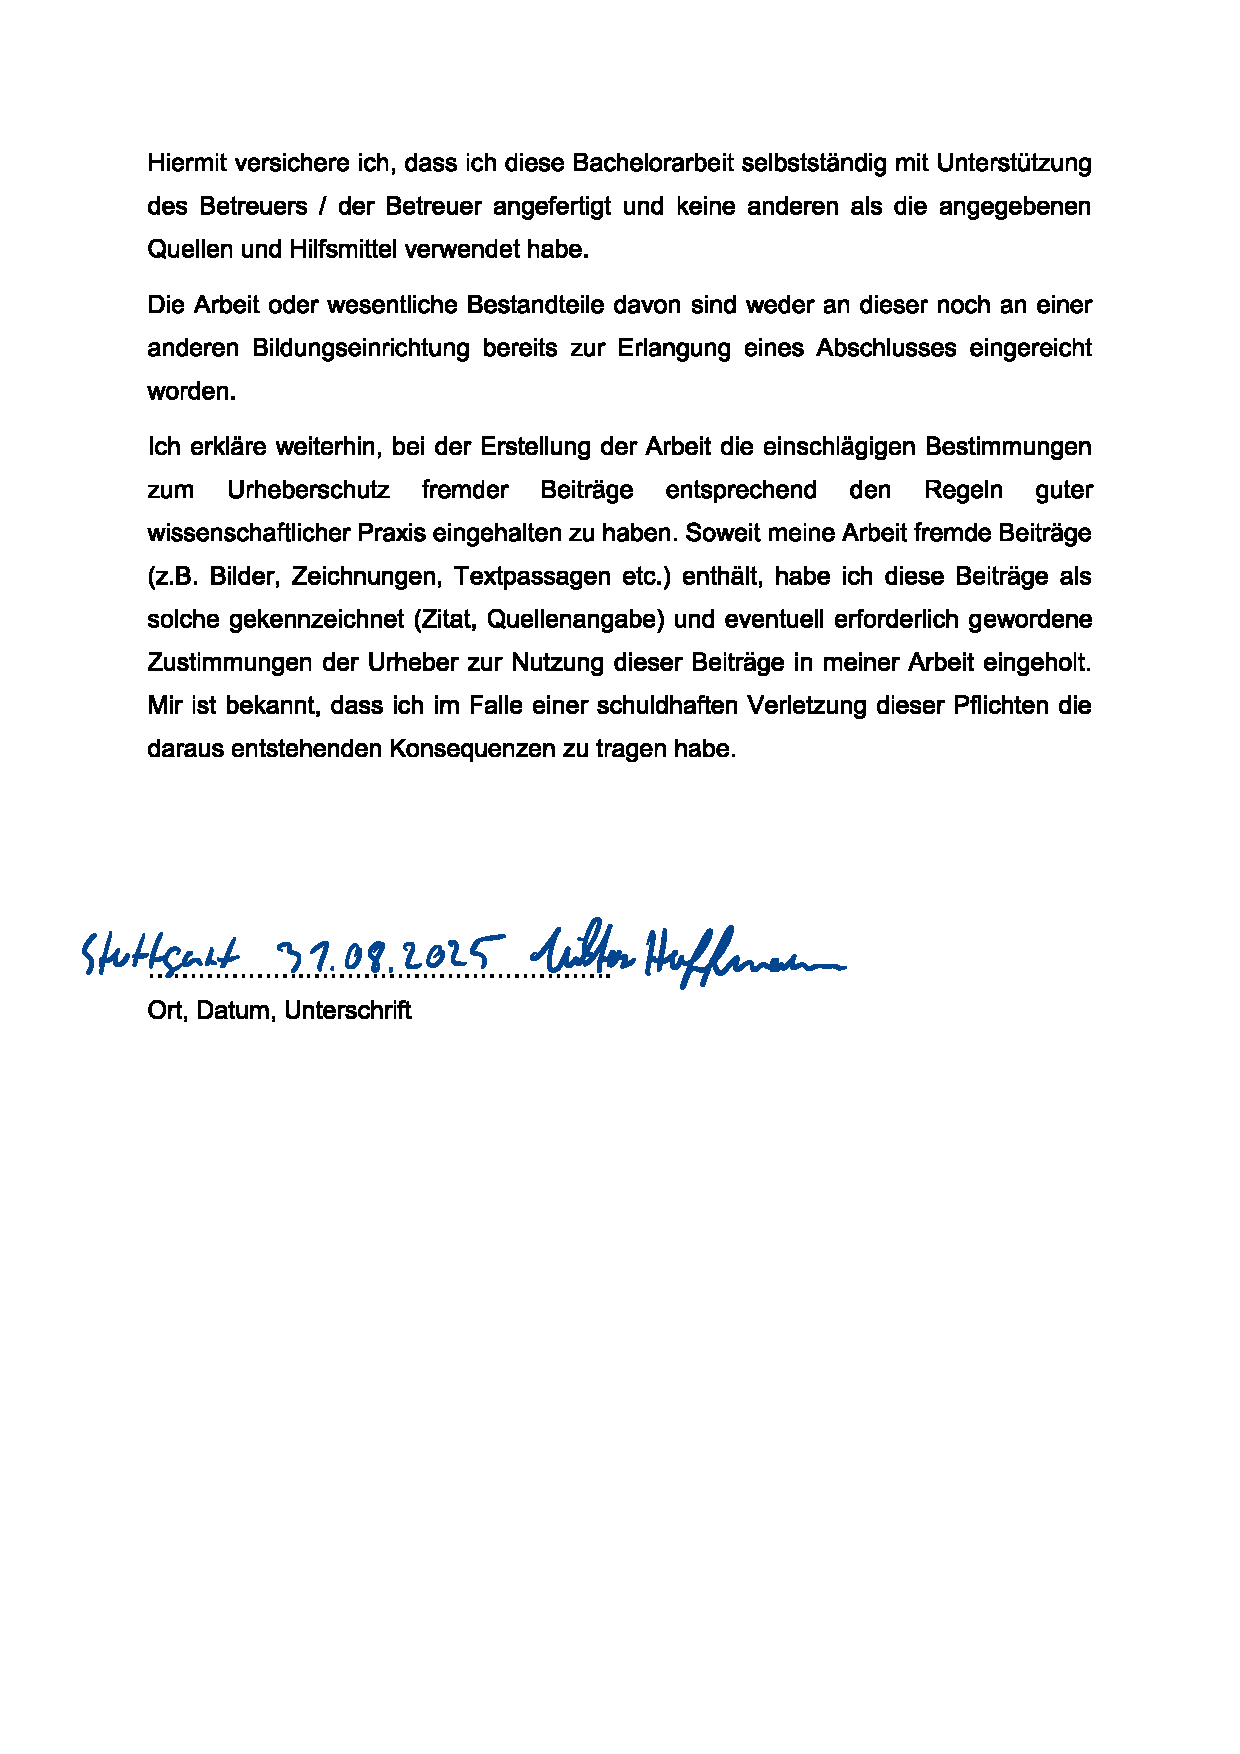
\includepdf{Text/Hoffmann_Bachelor_Eidesstatt.pdf}
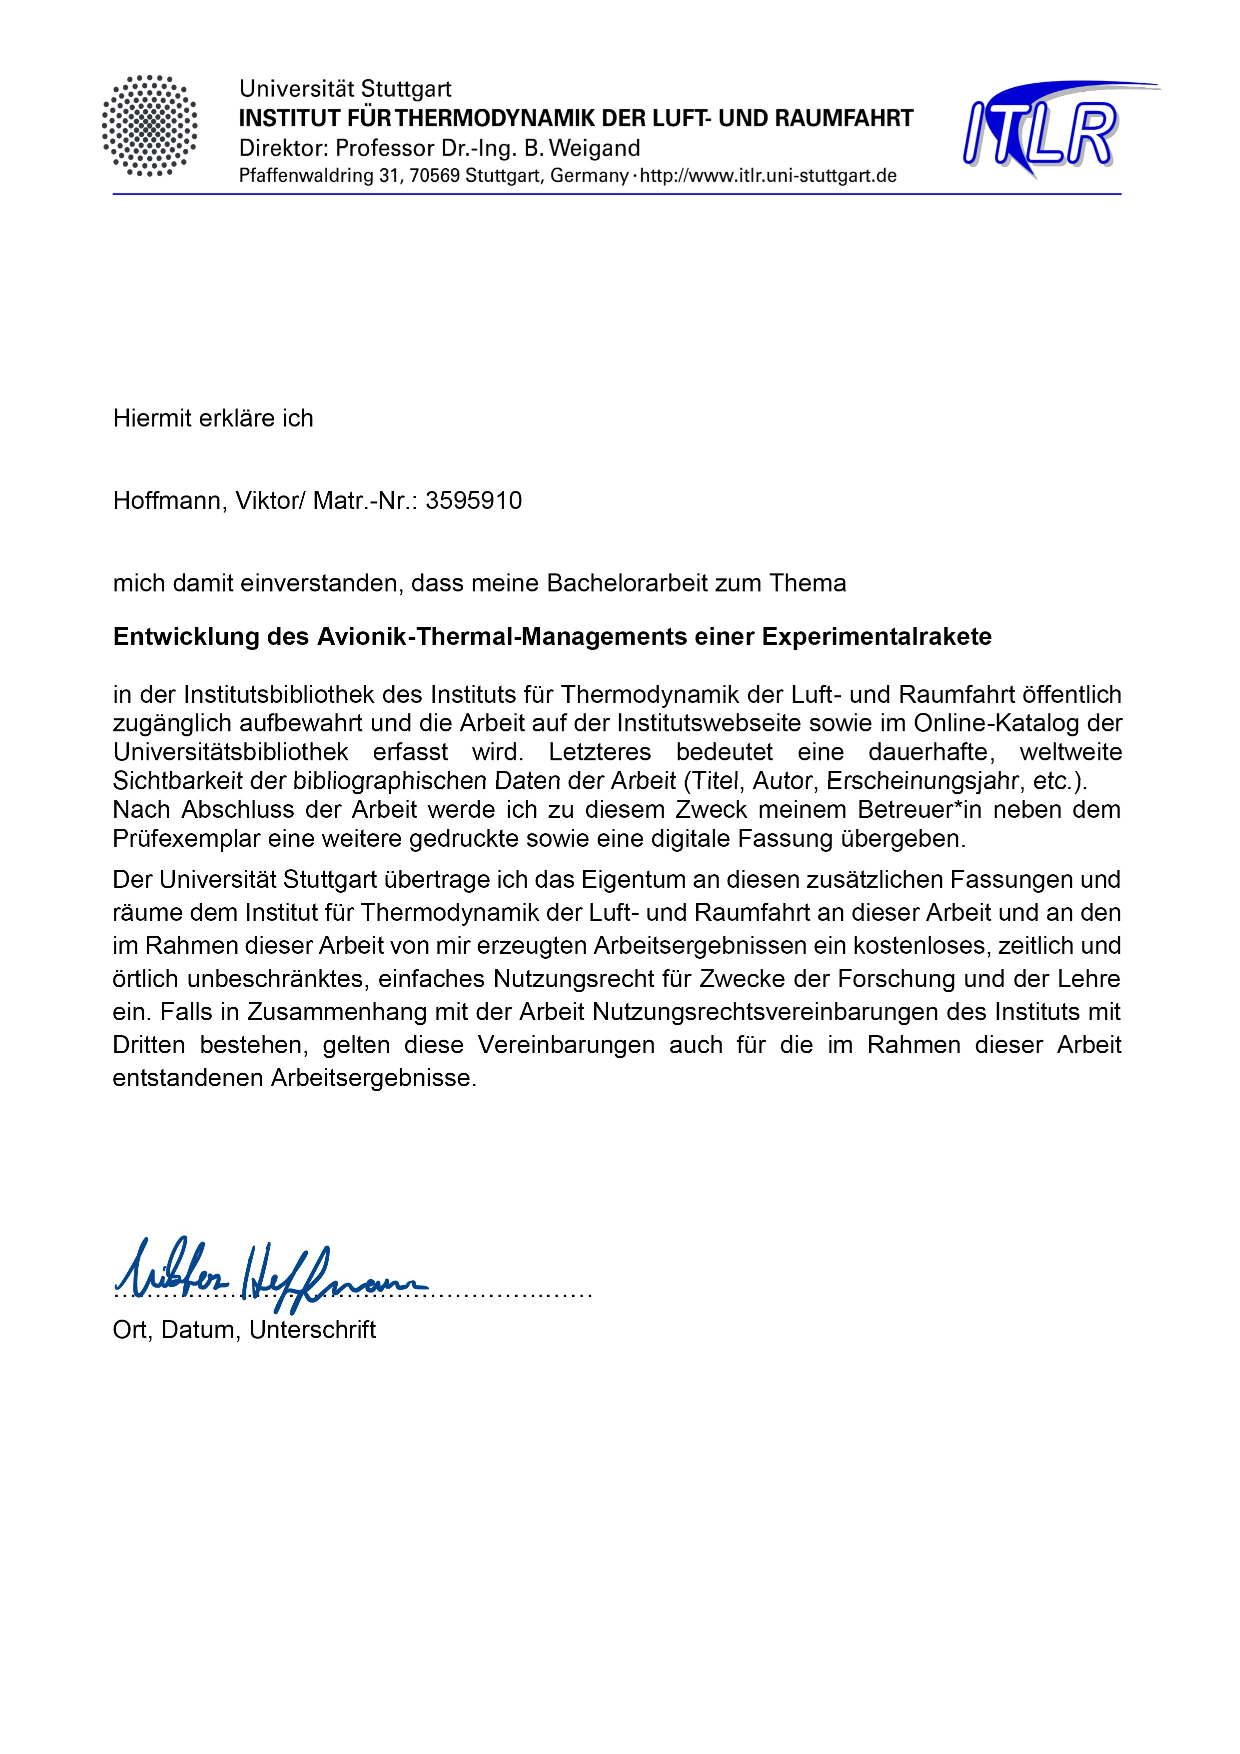
\includepdf{Text/Hoffmann_BA_Erklärung_Archivierung.pdf}

% erste Seite: Titelblatt (wird von ITLR erstellt)
% zweite Seite: leeres Blatt
% dritte Seite: Aufgabenstellung (wird von ITLR erstellt)
% vierte Seite: Erklärung (wird von ITLR erstellt, muss aber noch unterschrieben werden)

\pagenumbering{Roman}		% Am Anfang römische Seitenzahlen
% ----------- Abstract -------------------------------------------------------------
\newpage
\phantomsection		% Korrigiert die Hyperref-Verlinkungen
\addcontentsline{toc}{chapter}{Kurzzusammenfassung} %\addcontentsline
\chapter*{Kurzzusammenfassung} % * means not in table of content
\label{chap:Kurzzusammenfassung}

% ca. 150 Worte / Aufgabenstellung, Zielsetzung, verwendete Methoden, Ergebnisse kurz vorstellen, aber nicht diskutieren / Leser entscheidet hier, ob er die Arbeit für lesenswert hält

% deutsch
Für das Projekt \ac{blast} der Hochschulgruppe \ac{hyend} wird eine neue, kompakte und hochleistungsfähige Avionik entwickelt,
die unter extremen Flugbedingungen arbeitet. Die in dieser Arbeit entwickelte Kühlung muss leicht, zuverlässig, wiederverwendbar und für eine
maximale Gehäusetemperatur von $T_\mathrm{C} \leq \SI{89.15}{\celsius}$ während der gesamte Flugdauer ausgelegt sein.
Basierend auf den Anforderungen und Flugbedingungen
wurden drei Konzepte untersucht: reiner Radiator, reines \ac{pcm} und eine hybride Radiator-\ac{pcm}-Lösung. Die Vorauslegung
ergab, dass ein Radiator wegen Aerodynamischer Aufheizung ungeeignet ist. Die hybride Lösung ist möglich, jedoch durch geometrische
Verluste und hohe Luftwärmeströme der Vorauslegung nach mit \SI{4.256}{\kilogram} schwerer als ein einfaches \ac{pcm}
mit \SI{0.347}{\kilogram}. Simulationen der Außenströmung
bestätigten trotz angenommener Vereinfachungen die Vorauslegungsergebnisse mit einer Masse des hybriden Radiator-\ac{pcm} von \SI{1.654}{\kilogram}.
Die \ac{pcm} Simulation ergab eine Überschreitung der zulässigen Temperatur.

\chapter*{Abstract} % * means not in table of content
\label{chap:Abstract}
For the \ac{blast} project of the \ac{hyend} university group, a new, compact, and high-performance avionics system is being developed to
operate under demanding flight conditions. The cooling system developed in this work must be lightweight, reliable, reusable, and designed for a maximum
case temperature of $T_\mathrm{C} \leq \SI{89.15}{\celsius}$ for the entire flightduration.
Based on the requirements and flightconditions, three concepts were investigated: pure radiator, pure \ac{pcm}, and a hybrid radiator-\ac{pcm}
solution. Preliminary design showed that a radiator is unsuitable due to aerodynamic heating. The hybrid solution is feasible but, according to
the preliminary design, heavier at \SI{4.256}{\kilogram} due to geometric losses and high convective heat flux than a simple \ac{pcm} at
\SI{0.347}{\kilogram}. Simulations of the external flow confirmed the preliminary design results despite assumed
simplifications with a mass of the hybrid radiator \ac{pcm} of \SI{1.654}{\kilogram}. The \ac{pcm} Simulation resulted in temperatures
exceeding the design requirement.

% ----------- Verzeichnisse --------------------------------------------------------
% Inhaltsverzeichnis, Abbildungsverzeichnis, Tabellenverzeichnis, Nomenklatur 
\newpage
\tableofcontents	% Erstellt automatisch die Überschrift "Inhaltsverzeichnis" mit

% Tabellenverzeichnis
\newpage
\phantomsection		% Korrigiert die Hyperref-Verlinkungen
\pagestyle{VerzeichnisseNomenklatur}		% wie oben definiert
\addcontentsline{toc}{chapter}{Tabellenverzeichnis} 	% Eintrag ins InhaltsVZ
\listoftables

% Abbildungsverzeichnis
\newpage
\phantomsection		% Korrigiert die Hyperref-Verlinkungen
\addcontentsline{toc}{chapter}{Abbildungsverzeichnis}
\listoffigures				

% Symbolverzeichnis
\newpage
\phantomsection		% Korrigiert die Hyperref-Verlinkungen
\addcontentsline{toc}{chapter}{Symbolverzeichnis}
\chapter*{Symbolverzeichnis}
	
\subsection*{Lateinische Symbole}

\begin{supertabular}{p{10mm}p{3mm}p{20mm}p{3mm}l}
$T$ && \SI{}{\kelvin} && Temperatur\\
$c$ && \SI{}{\joule\per\kilogram\per\kelvin} && Spezifische Wärmekapazität\\
$h$ && \SI{}{\joule\per\kilogram} && Spezifische Schmelzenthalpie\\
$Q$ && \SI{}{\joule} && Wärme\\
$\dot{Q}$ && \SI{}{\watt} && Wärmestrom\\
$\dot{q}$ && \SI{}{\watt\per\meter\squared} && Wärmestromdichte\\ 
$m$ && \SI{}{\kilo\gram} && Masse\\
$A$ && \SI{}{\meter\squared} && Fläche\\
$S$ && \SI{}{\newton\per\meter\cubed} && Quellterm\\
$R$ && \SI{}{\kelvin\per\watt} && Wärmeleitwiederstand\\
\end{supertabular}


\subsection*{Griechische Symbole}

\begin{supertabular}{p{10mm}p{3mm}p{20mm}p{3mm}l}
$\rho$ && \SI{}{\kilogram\per\cubic\meter} && Dichte\\
$\lambda$ && \SI{}{\watt\per\meter\per\kelvin} && Wärmeleitfähigkeit\\
$\gamma$ && \SI{}{\per\kelvin} && Flüssigkeitsanteil\\
$\beta$ && && Wärmeausdehnungskoeffizient\\
$\varepsilon$ && && Emissionsgrad\\
$\alpha$ && && Absorptionsgrad\\
$\nabla$ && && Nablaoperator\\
\end{supertabular} 

\subsection*{Indizes}

\begin{supertabular}{p{10mm}p{3mm}p{20mm}p{3mm}l}
solidus && && Solidus Punkt des Phasenwechsels\\
liquidus && && Liquidus Punkt des Phasenwechsels\\
solid && && Feststoff Eigenschaften\\
liquid && && Flüssigstoff Eigenschaften\\
fus && && Schmelz Phasenwechsel\\
safety && && Mit Sicherheitsfaktor 1.5\\
senke && && Wärmesenke\\
total && && Totalgröße\\
ges && && Gesamt\\
p && && Konstanter Druck\\
J && && Sperrschicht\\
C && && Gehäuse\\
f && && Freistrom\\
w && && Wand\\
t && && Spektral integriert\\
s && && Solar\\
x && && Lokale Größe\\
r && && Recovery Größe\\
a && && adiabat\\
\end{supertabular} 

\subsection*{Konstanten}

\begin{supertabular}{p{10mm}p{3mm}p{50mm}p{3mm}l}
$\sigma$ && \SI{5.67e-8}{\watt\per\meter\squared\per\kelvin\tothe{4}} && Stefan-Boltzmann-Konstante\\
$\kappa$ && \SI{1.40}{} && Isentropenexponent der Luft\\
$\eta_0$ && \SI{18.27e-6}{\pascal\second} && Sutherlands-Formel Referenzviskosität\\
$T_0$ && \SI{291.15}{\kelvin} && Sutherlands-Formel Referenztemperatur\\
$C$ && \SI{120}{\kelvin} && Sutherland Konstante\\
\end{supertabular}

\newpage

%---Akronyme
\subsection*{Abkürzungen}
\begin{acronym}[BLAST]
\acro{pcm}[PCM]{Phase Change Material}
\acro{pcb}[PCB]{Printed Circuit Board}
\acro{blast}[BLAST]{Biliquid launch and Space Technology}
\acro{fcc}[FCC]{Flight Control Computer}
\acro{hyend}[HyEnD]{Hybrid Engine Development}
\acro{cfd}[CFD]{Computational Fluid Dynamics}
\acro{cht}[CHT]{Conjugate Heat Transfer}
\acro{pgs}[PGS]{Pyrolithic Graphite Sheet}
\acro{maxq}[max~Q]{Maximaler dynamischer Druck}
\acro{gse}[GSE]{Ground Support Equipment}
\acro{pcdu}[PCDU]{Power Control and Delivery Unit}
\acro{atm}[ATM]{Avionik-Thermal-Management}
\acro{rom}[ROM]{Reduced Order Model}
\acro{udf}[UDF]{User Defined Function}
\end{acronym}

% ----------- Verzeichnisse Ende-----------------------------------------------------
\newpage
\pagestyle{main}			% ab hier: normale Kopf- und Fußnoten
% ----------- Einleitung ------------------------------------------------------------
\chapter{Einführung}			
\label{sec:Introduction}
\pagenumbering{arabic}		%ab hier: arabische Seitenzahlen (Hauptteil)

% Problemstellung und Lösungsansätze, 2-3 Seiten / keine Ergebnisse & Folgerungen /

Die Avionik ist ein Grundstein jeder erfolgreichen Experimentalrakete. Ob es hierbei um Telekommunikation,
Datenerfassung oder auch aktive Steuerung und Regelung von
Instrumenten und dem Fahrzeug während des Flugs geht, kompakte Hochleistungsmikroelektronik ist immer gefragt und muss oft redundant ausgeführt sein.
Diese Elektronik, die zudem noch extremen Bedingungen ausgesetzt wird, kommt jedoch mit einer
substanziellen Wärmeleistung und Wärmestromdichte die bei mangelhafter Rücksicht zu reduzierter Lebensdauer der Avionik führt
oder sogar die Mission frühzeitig scheitern lässt.

Diese Arbeit befasst sich mit dem Lösungsansatz des dargestellten Problems für das Projekt \ac{blast} der studentischen Hochschulgruppe \ac{hyend},
wo eine neue Avionik entwickelt und ein \ac{atm} benötigt wird.

\section{Darstellung des Problems}

Das Thermal-Problem einer Experimentalrakete beginnt bereits lange vor dem eigentlichen Start. Oft muss nach Integration und
Befestigung der Rakete auf der Startvorrichtung und Verbindung mit dem \ac{gse} noch einige Stunden auf das Startfenster gewartet werden.
Während dieser Zeit steht die Rakete der Umwelt ausgesetzt in der Sonne und kann je nach Bedingungen 
unzulässige Temperaturen für die Elektronik erreichen. Da in dieser Phase eine Verbindung mit dem 
\ac{gse} besteht, kann Masse durch externe Kühlung währenddessen eingespart werden, weshalb in dieser Arbeit nur für die darauf folgende 
Flugphase das \ac{atm} entwickelt werden soll.
Da \ac{blast} für ein Apogäum über der Kármán-Linie (\SI{100}{\kilo\meter} über dem Meeresspiegel) entwickelt wird, sind während des Fluges extreme Umweltbedingungen
durch aerodynamische Aufheizung, Mikrogravitation und annäherndes Vakuum zu erwarten, die ein robustes \ac{atm} fordern.

In der Vergangenheit wurde bei \ac{hyend} oft die Avionik ohne Redundanz oder zusammen mit fertig gekaufter Avionik für 
missionskritische Aufgaben wie den Fallschirm-Auswurf ausgeführt. Beim Projekt \ac{blast} soll das vermieden werden, 
indem der selbst entwickelte \ac{fcc} in Dual-Duplex-Redundanz ausgelegt wird. Dementsprechend gibt es vier Computer, die
die selben Programme ausführen und den vierfachen Stromverbrauch gegenüber einfach ausgeführter Avionik haben. Hinzu kommen
weitere Kameras, Funkplatinen, Verstärker, Sensorplatinen etc., die jedoch keine redundante Ausführung haben.

\section{Zielsetzung der Arbeit}

Da es sich beim \ac{atm} um ein unterstützendes Subsystem handelt, soll besonders hohe Zuverlässigkeit gewährleistet werden, da trotz der
Redundanz des \ac{fcc} ein Ausfall der Kühlung zum Ausfall durch Überhitzung führen kann.
Des Weiteren ist Wiederverwendbarkeit, Kosten minimieren und besonders komplexe Integrations- und Vorbereitungsvorgänge
vermeiden eine Priorität.
Als letzte Anforderung soll wegen des begrenzten Massenbudgets der Avionik
besonders auf Leichtbau geachtet werden und die Masse des \ac{atm} soweit wie möglich minimiert werden.

\section{Lösungsweg}

Um ein geeignetes \ac{atm} zu entwickeln wird zunächst eine Auswahl an etablierten Lösungen aus der Luft- und Raumfahrtindustrie
getroffen, die die gestellten Anforderungen erfüllen können.

Diese werden in der Vorauslegung mithilfe eines \ac{rom} in Python ausgewertet, das eine dimensionsreduzierte Näherung des nichtlinearen Referenzmodells liefert, um eine erste Abschätzung der Leistungsfähigkeit zu erhalten.
Anschließend wird die Vorauslegung, soweit mit vorhandenen Rechenressourcen möglich, durch \ac{cht}-Simulationen mit Domänenreduktion
überprüft und mit diesen Ergebnissen verglichen.

%----------- Literaturrecherche -----------------------------------------------------
\newpage
\chapter{Grundlagen}
\label{chap:Grundlagen}			% durch \label{} später auf Element verweisen

In diesem Kapitel werden die Thermodynamischen, Chemischen und Numerischen Grundlagen die in dieser Arbeit angewandt wurden aufgelistet
und erläutert.
% Bücher, aber auch Paper etc. 

\section{Sensible Wärme}\label{sec:sensiblewaerme}
Unter sensibler Wärme versteht man die Eigenschaft von Masse durch eine Temperaturänderung Wärmeenergie zu absorbieren oder abzugeben. Dieses
Phänomen kann durch die Änderung der kinetischen Energie von den molekularen Teilchen im System erklärt werden. Durch das Einführen von
Wärmeenergie in ein System steigt die kinetische Energie der Teilchen:

\begin{equation}
    c = \frac{\Delta Q}{m \cdot \Delta T}
\end{equation}

$c$ beschreibt die spezifische Wärmekapazität, welche entweder bei konstantem Druck oder konstantem Volumen angegeben ist,
$Q$ ist die Wärmeenergie, $m$ die Masse und $T$ die Temperatur

Da Elektronik eine gewisse Eigenmasse hat und meist Teil einer größeren Baugruppe ist, gibt es durch die sensible Wärme eine Dämpfung
zu Temperaturänderungen, welche jedoch zeitlich von der Wärmeleitfähigkeit der Materialien abhängt.

\section{Latente Wärme}\label{sec:latentewaerme}

Im Gegenteil zur sensiblen Wärme ist latente Wärme, auch Umwandlungsenthalpie genannt, die Eigenschaft von Masse bei einem Phasenwechsel Wärmeenergie
zu absorbieren oder abzugeben, ohne dass sich dabei die Temperatur ändert. Das ist durch die Erhöhung der potentiellen Energie der Teilchen,
statt der kinetischen wie bei der sensiblen Wärme, zu verstehen. Effektiv erhöht sich die potentielle Energie durch Änderung der Bindungszustände.
Die Stoffkonstante der Umwandlungsenthalpie ist die spezifische Umwandlungsenthalpie $h$:

\begin{equation}
    h = \frac{\Delta Q}{m}
\end{equation}

Zu beachten ist, dass die Konvention der Schreibweise für die massenspezifische Fest-Flüssig Umwandlungsenthalpie spezifische Schmelzenthalpie ist,
aber für die massenspezifische Flüssig-Gas Umwandlungsenthalpie nur Verdampfungsenthalpie ist.

Die latente Wärme ist für die meisten Materialien im Fest-Flüssig Übergang um mindestens den Faktor 10 größer als die sensible Wärme bei
einem Grad Temperaturerhöhung. Genauso ist die Verdampfungsenthalpie vom Flüssig-Gas Übergang meist um etwa den Faktor 10 größer als die 
spezifische Schmelzenthalpie~\cite{fusion-vaporization}.

\section{Wärmeübertragung}\label{sec:waermeuebertragung}

Um Wärme innerhalb von einem System günstig zu verteilen, oder die Energie aus dem System zu entfernen, gibt es drei Mechanismen.

\subsection{Wärmestrahlung}\label{sec:strahlung}

Bei der Wärmestrahlung geben Teilchen beim aufnehmen oder abgeben kinetischer Energie eine Gewisse Menge an Energie in Form
von Elektromagnetischer Strahlung ab. Da die Strahlungsleistung von der vierten Potenz der Temperatur
abhängt, ist dieser Modus erst bei sehr hohen Temperaturen dimensionierend, kann jedoch im Vakuum dominant sein:

\begin{equation}
    \label{eq:radiation}
    \dot{Q}=\sigma\varepsilon A T^{4}
\end{equation}

$\dot{Q}$ ist der Wärmestrom, $\sigma$ die Stefan-Boltzmann-Konstante, $\varepsilon$ der Emissionsgrad, welcher von der Wellenlänge
abhängt, $A$ die Fläche und $T$ die Temperatur des Radiators.

\subsection{Wärmeleitung}\label{sec:waermeleitung}

Bei der Wärmeleitung wird Wärmeenergie in einem Körper durch diffusion der kinetischen Energie der Teilchen verteilt.
Die Wärmestromdichte $\dot{q}$ in einem Temperaturgradienten wird durch das Fourier-Gesetz beschrieben:

\begin{equation}
  \label{eq:fourier}
  \vec{\dot{q}} = -\lambda \nabla T
\end{equation}

Hier ist $\lambda$ die Wärmeleitfähigkeit des Materials.
Für eine eindimensionale Wand ergibt sich die Gleichung mit der Querschnittfläche $A$ und der Dicke $\Delta x$ zu:

\begin{equation}
  \label{eq:fourier_1d}
  \dot{Q} = \lambda A \frac{\Delta T}{\Delta x}
\end{equation}

Der Wärmeleitwiederstand $R$ für einen Körper lässt sich durch die Temperaturdifferenz pro Watt definieren:

\begin{equation}
  \label{eq:waermewiederstand}
  R = \frac{\Delta T}{\dot{Q}}
\end{equation}

\subsection{Konvektion}\label{sec:konvektion}

Bei der Konvektion wird Wärmeenergie durch Massenaustausch transportiert. Bei der erzwungenen Konvektion bekommt das Fluid durch äußere Kräfte
eine relative Geschwindigkeit, die zum Massenaustausch führt. Andererseits resultiert bei der natürlichen Konvektion nur die eigene
inhomogene Temperaturverteilung, durch beispielsweise eine anliegende heiße Wand, zu einem Temperaturanstieg und infolge dessen zu einem
Dichteanstieg, der in einem Beschleunigungsfeld zu Auftriebskräften und automatischer Bewegung des Fluids führt.
Für den Wärmeübergang zwischen Fluid und Festkörper ergibt sich:

\begin{equation}
    \dot{Q}=\alpha A \Delta T 
\end{equation}

Hier ist $\alpha$ der Wärmeübergangskoeffizient.
Für den spezifischen Wärmestrom zwischen Fluid und Wand folgt daraus:

\begin{equation}
  \label{eq:qdot_freestream}
  \dot{q} = \alpha \ (T_{\infty} - T_\text{w})
\end{equation}

Der Wärmeübergangskoeffizient $\alpha$ kann aus der Nußelt-Beziehung für Längsangeströmte ebene Platte genommen. Diese lautet
für laminare Grenzschichten im Gültigkeitsbereich $\text{Re} < \text{Re}_k \left(\text{Re}_k \approx 5 \cdot 10^5\right)$ und $0,6 \leq \text{Pr} \leq 2000$:

\begin{equation}
  \label{eq:nusselt_laminar}
  \text{Nu}_x = \frac{\alpha_x x}{\lambda} = \num{0,332} \ \text{Pr}^{\frac{1}{3}} \ \text{Re}_x^{\frac{1}{2}}
\end{equation}

für turbulente Grenzschichten mit Gültigkeitsbereich: $5 \cdot 10^5 \leq \text{Re}_L \leq 10^7$ und $ 0,6 \leq \text{Pr} \leq 2000$ lautet die Gleichung:

\begin{equation}
  \label{eq:nusselt_turbulent}
  \text{Nu}_x = \frac{\alpha_x x}{\lambda} = \num{0,0296} \ \text{Re}_x^{0,8} \ \text{Pr}^{\frac{1}{3}}
\end{equation}

Für die Reynolds-Zahl und Prandtl-Zahl werden die folgenden zwei Gleichungen verwendet:

\noindent\begin{minipage}{.5\linewidth}
  \begin{equation}
    \label{eq:reynolds}
    Re_x = \frac{U \rho x}{\eta}
  \end{equation}
\end{minipage}%
\begin{minipage}{.5\linewidth}
  \begin{equation}
    \label{eq:prandtl}
    Pr = \frac{c_p \eta}{\lambda}
  \end{equation}
\end{minipage}

Die Dynamische Viskosität $\eta$ wird mittels der Sutherlands-Formel berechnet, wobei $\eta_0$, $C$ und $T_0$ Konstanten für Luft sind:

\begin{equation}
  \label{eq:dynamische_viskositaet}
  \eta = \eta_0 \frac{T_0 + C}{T_{\infty} + C} {\left( \frac{T_{\infty}}{T_0} \right)}^{\frac{3}{2}}
\end{equation}

Eine Strömung ist im Überschallbereich, wenn ihre Machzahl größer als 1 ist:

\begin{equation}
  \label{eq:machzahl}
  Ma = \frac{U}{a}
\end{equation}

Wobei $U$ die Strömungsgeschwindigkeit und $a$ die lokale Schallgeschwindigkeit ist. Im Überschallbereich treten verschiedene
Effekte durch die Kompressibilität der Strömung auf, wie etwa durch Stoßwellen mit sprunghaftem Anstieg von Temperatur und Druck,
oder Expansionsfächern mit sprunghaftem Abfall dieser Größen. Auch die adiabate Kompression resultiert in Temperaturerhöhungen.
Die in einer Grenzschicht erreichte Temperatur durch Reibung
ist immer kleiner als die Totaltemperatur $T_{\infty} < T_r < T_\mathrm{total}$, da die kinetische Energie nur teilweise in innere Energie
umgewandelt wird und somit mit dem Recovery-Faktor $r$ skaliert ist:

\begin{equation}
  \label{eq:recovery_temperatur}
  T_r = T_{\infty} \left( 1 + r \frac{\kappa - 1}{2} \text{Ma}^2 \right)
\end{equation}

Der Recovery-Faktor kann mittels der folgenden Gleichung berechnet werden:

\begin{equation}
  \label{eq:recovery_faktor}
  r = \frac{2}{\left( \kappa - 1 \right) \mathrm{Ma_{\infty}}^2} \left( \frac{T_\mathrm{a_{w}}}{T_{\infty}} - 1 \right) \approx
  \begin{cases}
    \sqrt[3]{\text{Pr}} & \text{für turbulente Grenzschicht}\\
    \sqrt{\text{Pr}} & \text{für laminare Grenzschicht}
  \end{cases}
\end{equation}

In einer kompressiblen Strömung bei $\mathrm{Ma} > 0.3$ wird somit $T_{\infty}$ aus \ref{eq:qdot_freestream} zu $T_\text{r}$:

\begin{equation}
  \label{eq:qdot_recovery}
  \dot{q} = \alpha \ (T_r - T_w)
\end{equation}

\section{Simulation}
\section*{Aerodynamische Aufheizung}

Die numerische Strömungssimulation (\ac{cfd}) ist ein Verfahren zur Berechnung von Strömungs- und Wärmeübergangsprozessen
mithilfe numerischer Methoden. \ac{cfd} erlaubt die Untersuchung komplexer Geometrien und Betriebsbedingungen,
die experimentell nur schwer oder gar nicht möglich sind. Ziel ist es, die Navier-Stokes-Gleichungen in differentieller Form auf einer
diskreten Gitterstruktur zu lösen. Diese Erhaltungsgleichungen sind die Massenerhaltung:

\begin{equation}
  \label{eq:navier_massenerhaltung}
  \frac{\partial \rho}{\partial t} + \nabla \left( \rho \vec{u} \right) = 0
\end{equation}

Impulserhaltung:

\begin{equation}
  \label{eq:navier_impulserhaltung}
  \frac{\partial \left( \rho \vec{u} \right)}{\partial t} + \nabla \left( \rho \vec{u} \vec{u} \right) = -\nabla p + \nabla \tau + \rho \vec{g}
\end{equation}

und Energieerhaltung:

\begin{equation}
  \label{eq:navier_energieerhaltung}
  \frac{\partial \left(\rho \vec{u}\right)}{\partial t} + \nabla \left[\left(\rho E + p\right)\vec{u}\right] = \nabla \left(k \nabla T\right) + \Phi
\end{equation}

Hier sind $\rho$ die Dichte, $\vec{u}$ der Geschwindigkeitsvektor, $p$ der statische Druck, $\tau$ der Spannungstensor,
$\vec{g}$ die Gravitationsbeschleunigung, $E$ die spezifische Gesamtenergie, $T$ die Temperatur, $k$ die Wärmeleitfähigkeit
und $\Phi$ der viskose Dissipationsterm.

Eine wichtige Metrik bei der Behandlung von Grenzschichten in viskosen Fluiden ist der Dimensionslose Wandabstand:

\begin{equation}
  \label{eq:yplus}
  y^+ = \frac{\rho u_{\tau} y}{\eta}
\end{equation}

Dieser wird mittels des Abstandes $y$ der ersten Zelle die an der Wand anliegt, der Schubspannung an der Wand $\tau_w$ und der daraus resultierenden Schubspannungsgeschwindigkeit $u_{\tau}$ berechnet:

\noindent\begin{minipage}{.5\linewidth}
  \begin{equation}
    \label{eq:schubspannung}
    \tau_w = \eta \left.\frac{\partial u}{\partial y}\right|_{y=0} = \frac{1}{2} \rho U_{\infty}^{2} C_f
  \end{equation}
\end{minipage}%
\begin{minipage}{.5\linewidth}
  \begin{equation}
    \label{eq:schubspannung_geschwindigkeit}
    u_{\tau} = \sqrt{\frac{\tau_w}{\rho}}
  \end{equation}
\end{minipage}

Hierbei ist $\eta$ die dynamische Viskosität, $\left.\frac{\partial u}{\partial y}\right|_{y=0}$ der Geschwindigkeitsgradient senkrecht zur Wand
und $C_f$ der Reibungsbeiwert.
Für $C_f$ gibt es folgende empirische Näherungen~\cite{Anderson-2017}:

\begin{minipage}{.5\linewidth}
  \begin{equation}
    \label{eq:reibungsbeiwert_laminar}
    C_f \approx \frac{0.664}{\sqrt{{Re}_x}} \hspace{0.5em} \mathrm{bei} \hspace{0.5em} Re \leq \SI{5e5}{}
  \end{equation}
\end{minipage}%
\begin{minipage}{.5\linewidth}
  \begin{equation}
    \label{eq:reibungsbeiwert_turbulent}
    C_f \approx \frac{0.0592}{{Re}_x^{1/5}} \hspace{0.5em} \mathrm{bei} \hspace{0.5em} Re > \SI{5e5}{}
  \end{equation}
\end{minipage}

Für Wärmeübertragungsprobleme an Wänden muss man die Zellhöhe so wählen, dass man im Bereich $y^+ \leq 1$ bleibt.

\section*{PCM}
Um Temperatur- und Phasenabhängige Eigenschaften für die \ac{cht}-Simulation von \ac{pcm} darzustellen, sowie Zeitabhängige Auftriebsterme, kommen weitere Modelle dazu,
die in ANSYS Fluent nicht implementiert sind. Dafür wird eine in C programmierte \ac{udf} verwendet, die in Fluent direkt importiert
und kompiliert werden kann.
Die Boussinesq-Approximation modelliert den Auftrieb infolge von geringen Dichteänderungen. Für den Auftrieb
in dem Impulsterm ergibt sich somit~\cite{akamcae-udf}:

\begin{equation}
  \label{eq:udf_bouss}
  S = -\rho_0 \, g_\text{eff}(t)\,\beta\,(T-T_0)
\end{equation}

Hierbei ist $S$ der Quellterm, $\beta$ der Wärmeausdehnungskoeffizient, $g_\text{eff}(t)$ die effektive, Zeitabhängige Beschleunigung,
$T_0$ und $\rho_0$ die Referenz-Temperatur und Dichte. Diese Approximation kann den Rechenaufwand erheblich verringern und ist für folgende Bedingungen gültig:

\noindent\begin{minipage}{.5\linewidth}
  \begin{equation}
    \label{eq:bossinesque_bedingung1}
    \frac{\Delta T}{T_0} \ll 1
  \end{equation}
\end{minipage}%
\begin{minipage}{.5\linewidth}
  \begin{equation}
    \label{eq:bossinesque_bedingung2}
    \text{Ma} \ll 1
  \end{equation}
\end{minipage}

ANSYS Fluent verwendet zur Modellierung des Schmelzbereiches ein internes \allowbreak Enthalpy-Porosity-Modell, welches das \ac{pcm} als poröses Material
mit diskreter Fest- und Flüssigphase ansieht. Hierfür ist die Dichte $\rho$ notwendig und kann in Abhängigkeit des Flüssigkeitsanteils $\gamma$ berechnet werden.
Zwischen der Dichte der Flüssig- und Feststoffphase wird linear interpoliert~\cite{akamcae-udf}:

\begin{equation}
  \label{eq:udf_dichte}
  \rho(\gamma) = \left(1- \gamma\right) \rho_\text{solid} + \gamma \rho_\text{liquid} \qquad \gamma \in [0,1]
\end{equation}

Die spezifische Wärmekapazität ergibt sich im Schmelzbereich durch eine Dichtegewichtete Mischung~\cite{akamcae-udf}:

\begin{equation}
  \label{eq:udf_cp}
    c_p(T)=
  \begin{cases}
    c_{p,\mathrm{solid}}, & T < T_\mathrm{solid},\\[6pt]
    \dfrac{(1-\gamma)\,\rho_\mathrm{solid}\,c_{p,\mathrm{solid}} + \gamma\,\rho_\mathrm{liquid}\,c_{p,\mathrm{liquid}}}
          {(1-\gamma)\,\rho_\mathrm{solid} + \gamma\,\rho_\mathrm{liquid}}, & T_\mathrm{solid} \le T \le T_\mathrm{liquid},\\[12pt]
    c_{p,\mathrm{liquid}}, & T > T_\mathrm{liquid}.
  \end{cases}
\end{equation}

Die Wärmeleitfähigkeit $\lambda$ im Schmelzbereich hingegen lässt sich direkt berechnen~\cite{akamcae-udf}:

\begin{equation}
  \label{eq:udf_lambda}
  \lambda(\gamma)= (1-\gamma)\,\lambda_{\mathrm{solid}} + \gamma\,\lambda_{\mathrm{liquid}}
\end{equation}

Die Dynamische Viskosität $\eta$ wird hier, anders als für Luft in der Vorauslegung \ref{eq:dynamische_viskositaet}, mittels eines empirischen
Polynomfit~\cite{akamcae-udf} abhängig von der Temperatur berechnet:

\begin{equation}
  \label{eq:udf_mu}
  \eta(T)= \left(9\times 10^{-4}\,T^{2} - 0.6529\,T + 119.94\right)\times 10^{-3}
\end{equation}

In der verwendeten Software ANSYS Fluent werden diese Gleichungen über die Finite-Volumen-Methode gelöst. Dabei werden die Erhaltungsgleichungen
über diskrete Kontrollvolumina integriert, wodurch für jede Zelle ein algebraisches Gleichungssystem entsteht. Dieses
wird iterativ gelöst, bis vorgegebene Konvergenzkriterien erfüllt sind.

% ----------- Methodik --------------------------------------------------------------
\chapter{Vorauslegung}
\label{chap:Vorauslegung}



Die Flugdaten kommen aus einer Trajektoriensimulation aus dem Simulationsprogramm OpenRocket, welche vom Triebwerk-Subsystem durchgeführt wurde.
Diese Flugdaten in Abbildung \ref{fig:flugdaten_trajektoriensimulation} bilden eine Maximalabschätzung der Aerodynamischen Aufheizung und Flugdauer durch
maximale Schub-Kraft und Dauer mit \SI{8}{\kilo\newton} für \SI{43}{\second}, die von \ac{blast} erreicht werden können.

\section{Anforderungen}

Da die Kühlung zeitgleich zu der Avionik entwickelt wurde, musste auf eine genaue Analyse aller Komponenten der Avionik verzichtet werden.
Stattdessen wurde anhand der bereits festgelegten Elektronik wie etwa dem Mikrocontroller STM32H743ZGT6, der auf den redundanten Flugcomputern verwendet wird,
die Auslegung durchgeführt.
Aus dem Datenblatt des Mikrocontrollers folgt eine maximale Sperrschichttemperatur von $T_\text{J} = \SI{125}{\degreeCelsius}$~\cite{STM32}
und ein Sperrschicht-Gehäuse Wärmeleitwiederstand von $\Theta_\text{JC} = \SI{23.9}{\degreeCelsius\per\watt}$~\cite{STM32}. Mit einem konservativen
Sicherheitsfaktor von 1.5, um bisher unbekannte Bauteile zu berücksichtigen, folgt daraus $\Theta_\text{JC,safety} = \SI{35.85}{\degreeCelsius\per\watt}$
und eine maximale Gehäusetemperatur von $T_\text{C} = \SI{89.15}{\degreeCelsius}$. Im Kontext der Elektronik ist mit Gehäuse immer die
Oberseite der elektronischen Komponente gemeint.
Die Kühlung soll außerdem eine hohe Zuverlässigkeit haben, welche durch Verwendung von ausschließlich passiven Bauteilen gewehrleistet wird.
Dadurch kann aufwendiges und teures testen und verifizieren von aktiven Bauteilen mit mechanischer oder elektrischer Funktion vermieden werden und es besteht bei
nicht nominalen Flügen eine geringere Ausfallwahrscheinlichkeit durch die inherent größeren Toleranzen passiver Bauteile.

Dem Energieerhaltungssatz nach haben der \ac{fcc}, die Kameras und weitere Elektronik die keine Leistung abgibt, gegenüber etwa
der \ac{pcdu} und Funkplatine welche Leistung in Form von Strom und elektromagnetischer Strahlung abgeben, einen Wirkungsgrad von
\SI{0}{\percent}, da Logikoperationen physikalisch gesehen keine Arbeit sind. Resultierend wird der komplette Stromverbrauch
in Wärme umgewandelt.

\begin{table}
  \centering
  \caption{Leistung der Avionik}\label{tab:avionik_leistung}

  \begin{tabular}{lp{4cm}ll}
    \toprule[1pt]
    Komponente & Spannung \& Strom & Wirkungsgrad & Wärmestrom \\
    \midrule[0.5pt]

    STM32H743ZGT6 &
      \mbox{$V_\text{DD}=\SI{3.3}{\volt}$},\newline
      $I_\text{DD}=\SI{536}{\milli\ampere}$~\cite{STM32} &
      $\approx \SI{0}{\percent}$ & \SI{1.769}{\watt} \\
    $\dot{Q}_\text{ges}$ & & & \SI{7.075}{\watt}\\

    \midrule[0.5pt]
    RunCam Split 4 V2 &
      \mbox{$V_\text{DD}=\SI{5}{\volt}$},\newline
      $I_\text{DD}=\SI{450}{\milli\ampere}$~\cite{RunCam-Split4V2} &
      $\approx \SI{0}{\percent}$ & \SI{2.25}{\watt} \\
    $\dot{Q}_\text{ges}$ & & & \SI{9}{\watt}\\

    \midrule[0.5pt]
    Thebe-II &
      \mbox{$V_\text{DD}=\SI{3.6}{\volt}$},\newline
      $I_\text{DD}=\SI{500}{\milli\ampere}$~\cite{WE-ThebeII-UM-2024} &
      $\approx \SI{30}{\percent}$~\cite{WE-ThebeII-UM-2024} & \SI{1.3}{\watt} \\

    \midrule[0.5pt]
    \ac{pcdu} & & $\approx \SI{30}{\percent}$ & \SI{9.3}{\watt} \\

    \midrule[0.5pt]
    \midrule[0.5pt]
    $\dot{Q}_\text{ges, safety}$ & & & \SI{40}{\watt} \\

    \bottomrule[1pt]
  \end{tabular}
\end{table}

Die Leistung der Avionik in Tabelle~\ref{tab:avionik_leistung} ergibt sich durch den Maximalverbrauch der \ac{fcc} mikrocontroller
(STM32H743ZGT6) bei maximaler clock rate (\SI{400}{\mega\hertz}) und vollständig aktiver Peripherie, der Kameras und einer
Abschätzung der restlichen Komponenten, für die keine exakten Werte vorhanden sind. Der aus Tabelle~\ref{tab:avionik_leistung} resultierende gesamte Wärmestrom
der Avionik mit \SI{40}{\watt} ist mit einem gewöhnlichen Laptop vergleichbar.

\begin{figure}
    \centering

    % Column 1, Row 1
    \begin{subfigure}{0.48\textwidth}
        \centering
        \includegraphics[width=\linewidth]{../../Code/acceleration_over_time.pdf}
        \caption{Beschleunigung während Flug}
        \label{fig:acceleration_over_time}
    \end{subfigure}
    \hfill
    % Column 2, Row 1
    \begin{subfigure}{0.48\textwidth}
        \centering
        \includegraphics[width=\linewidth]{../../Code/altitude_over_time.pdf}
        \caption{Flughöhe}
        \label{fig:altitude_over_time}
    \end{subfigure}

    \vspace{1em}

    % Column 1, Row 2
    \begin{subfigure}{0.48\textwidth}
        \centering
        \includegraphics[width=\linewidth]{../../Code/pressure_over_time.pdf}
        \caption{Statischer Luftdruck während Flug}
        \label{fig:pressure_over_time}
    \end{subfigure}
    \hfill
    % Column 2, Row 2
    \begin{subfigure}{0.48\textwidth}
        \centering
        \includegraphics[width=\linewidth]{../../Code/temperature_over_time.pdf}
        \caption{Statische Lufttemperatur während Flug}
        \label{fig:temperature_over_time}
    \end{subfigure}

    \vspace{1em}

    % Column 1, Row 3
    \begin{subfigure}{0.48\textwidth}
        \centering
        \includegraphics[width=\linewidth]{../../Code/velocity_over_time.pdf}
        \caption{Geschwindigkeit während Flug}
        \label{fig:velocity_over_time}
    \end{subfigure}
    \hfill
    % Column 2, Row 3
    \begin{subfigure}{0.48\textwidth}
        \centering
        \includegraphics[width=\linewidth]{../../Code/dynp_during_flight.pdf}
        \caption{Dynamischer Druck während Flug}
        \label{fig:dynp_over_time}
    \end{subfigure}

    \caption{Flugdaten der Trajektoriensimulation}\label{fig:flugdaten_trajektoriensimulation}
\end{figure}

\section{Thermale Schnittstelle}\label{sec:thermale_schnittstelle}

Um mit der Abwärme der Avionik umgehen zu können, muss sie effektiv gesammelt und abtransportiert werden.
Oft werden in der Luft- und Raumfahrtindustrie Kühlkreisläufe mit einem Arbeitsfluid verwendet, etwa bei der Internationalen Raumstation~\cite{ISS-ATCS}.
Diese benötigen jedoch meist bewegliche Bauteile wie Pumpen, welche die Ausfallwahrscheinlichkeit erhöhen. Alternativ gibt es auch
Möglichkeiten durch erzwungene Konvektion ein Arbeitsfluid anzutreiben oder Materialien mit hoher Wärmeleitfähigkeit
zu verwenden. Beide Methoden bieten in Kombination eine leichte Integrierbarkeit und geringen Wärmeleitwiederstand,
ohne Bewegliche Teile zu verwenden.

Das Thermale Interface wird auf Systemebene analysiert, da eine Entwicklung auf \ac{pcb} Ebene wie bereits erläutert nicht
möglich ist, ohne die vollständig entwickelte Elektronik.

\subsection{Heatpipes}\label{sec:waermerohre}

Heatpipes (Wärmerohre) sind eine Möglichkeit durch erzwungene Konvektion Wärme zu transportieren. Reguläre Heatpipes
sind vollständig geschlossene Rohre mit einer Flüssigkeit im inneren und einer Kapillarstruktur an der Innenwand,
so dass ein freier Kanal in der Mitte bleibt. Bei der Wärmequelle
verdampft die Flüssigkeit aus der Kapillarstruktur und bei der Wärmesenke kondensiert sie wieder, wodurch der resultierende Massenstrom einen
Kreislauf bildet. Besonders effektiv sind Heatpipes durch die Nutzung der Verdampfungsenthalpie beim Flüssig-Gas Übergang an der Wärmequelle,
wodurch sehr hohe Wärmestromdichten erreicht werden können. Eine Schematische Darstellung einer Heatpipe kann in Abbildung~\ref{fig:waermerohr}
gesehen werden.

Eine Weiterentwicklung davon sind Loop Heatpipes die, wie der Namen bereits impliziert einen Kreislauf bilden, indem es eine
separate Flüssig- und Dampfleitung gibt, welche jeweils am Verdampfer und Kondensator miteinander verbunden sind.
Besonders von Vorteil sind Loop Heatpipes, wenn größere Distanzen überbrückt werden müssen, oder eine relativ zuverlässige
Funktion unabhängig von Orientierung und Gravitation gebraucht wird. Aufgrund der erhöhten Komplexität von Loop Heatpipes, der Möglichkeit
die Orientierung der Heatpipes frei zu bestimmen, den relativ geringen Distanzen innerhalb der Avionik-sektion und dem Mangel an Kommerziell erhältlichen
Loop Heatpipes wird eine reguläre Heatpipe gewählt.


\begin{figure}
  \centering
  \begin{tikzpicture}
    \draw[thick] (-5,0) arc [start angle=90, end angle=270, x radius=1.5cm, y radius= 1.5cm]; % Kappen
    \draw[thick] (5,0) arc [start angle=90, end angle=-90, x radius=1.5cm, y radius= 1.5cm];

    \draw[thick] (-5,0) -- (5,0); % hülle
    \draw[thick] (-5,-3) -- (5,-3);

    \draw[dashed] (-5,0) rectangle (5,-1); % Wick Abgrenzung
    \draw[dashed] (-5,-2) rectangle (5,-3);

    \draw[->, thick, -{Stealth[length=0.25cm]}] (-1,-1.75) -- node [midway, above] {Dampfstrom} (1,-1.75); % Dampf Pfeil
    \draw[->, thick, -{Stealth[length=0.25cm]}] (1,-2.75) -- node [midway, above] {Flüssigstrom}(-1,-2.75); % Flüssigkeitspfeil
    \draw[->, thick, -{Stealth[length=0.25cm]}] (1,-0.5) -- (-1,-0.5); % Flüssigkeitspfeil

    \node at (-4,-4) [style={single arrow, draw}, minimum height=0.5cm, minimum width=1.5cm, shape border rotate=90, thick]{$\dot{Q}$}; % Wärmestrom pfeil
    \node at (4,-3.75) [style={single arrow, draw}, minimum height=0.5cm, minimum width=1.5cm, shape border rotate=270, thick]{$\dot{Q}$}; % Wärmestrom pfeil
    
    \draw[->, thick, -{Stealth[length=0.25cm]}] (-4,0.25) node [above=1pt] {Kapillarstruktur} -- (-3,-0.5); % Kapillar Pfeil
    \draw[->, thick, -{Stealth[length=0.25cm]}] (-4,0.25) -- (-3,-2.5);
  \end{tikzpicture}
  \caption{Heatpipe Aufbau und Funktionsweise}\label{fig:waermerohr}
\end{figure}

Ein wichtiger Aspekt von Heatpipes ist, dass der Wärmeleitwiederstand durch Biegungen und Anbindung von mehreren Quellen um bis zu \SI{100}{\percent}
steigen kann \cite{Mooney-2020}. Auch wenn Heatpipes konvektiv arbeiten ist bei deren Wärmeübertragung vom Wärmeleitwiederstand die Rede.
Des weiteren hängt besonders bei regulären Heatpipes der Wärmeleitwiederstand von der effektiven Beschleunigung ab,
da die höhere Dichte der Flüssigphase eine beschleunigende Wirkung auf die Konvektion hat, wenn die Wärmequelle unten orientiert ist. Sollte die Heatpipe jedoch
\glqq überkopf \grqq{} arbeiten, sodass die Wärmequelle oben orientiert ist, muss die Konvektion gegen die Beschleunigung arbeiten und verliert Leistung bzw. hat
einen erhöhten Wärmeleitwiederstand.

Ausgewählt wurde die QG-SHP-D5-400MN Heatpipe von Quick-Ohm Küpper \& Co. GmbH aus Kupfer mit Mesh-Gewebe als Kapillarstruktur von \SI{400}{\milli\meter} Länge und
\SI{5}{\milli\meter} Durchmesser. Diese Heatpipe kann eine Leistung von \SI{40}{\watt} übertragen.

Weiterhin wird die Heatpipe als \ac{rom} mit einem einfachen Widerstand ersetzt, der dem Wärmeleitwiederstand von $R_\mathrm{Heatpipe} = \SI{0,3}{\kelvin\per\watt}$ aus dem Datenblatt~\cite{QuickOhm-Heatpipe-5x400} entspricht.
Dadurch wird eine sehr komplexe Modellierung abhängig von Temperaturen, Biegungen, Ausrichtung, Beschleunigung und Anzahl an Wärmequellen sowie deren Leistung und Positionen vermieden.

\subsection{Wärmeleitbänder}\label{sec:waermebaender}

Um die Elektronik mit dem Heatpipe zu verbinden werden Wärmeleitbänder aus verschiedenen Materialien analysiert.
Wärmeleitbänder sind flexible Verbindungsteile mit hoher Wärmeleitfähigkeit die Wärmebrücken zwischen mehreren Bauteilen gewährleisten.
\ac{pgs} ist gegenüber herkömmlichen Materialien besonders interessant durch die extrem hohe Wärmeleitfähigkeit innerhalb der Ebene,
da diese der Ebene von der Molekülstruktur des Graphit entspricht. Außerdem ist es ein relativ flexibles Material, bei einer üblichen Dicke von $\approx \SIrange{10}{100}{\micro\meter}$.
Ein Nachteil von \ac{pgs} ist die im Kontrast zur Ebene sehr niedrige Wärmeleitfähigkeit durch die Ebene, infolge von wenigen
molekularen Brücken zwischen den Gitterstrukturen. Dementsprechend wird \ac{pgs} und andere Arten von Graphit Folien hauptsächlich zur
Wärmeverteilung auf der Oberfläche von Bauteilen verwendet um Wärmestromdichten zu verringern und homogenere Temperaturverteilungen zu erreichen.

Das effektive erhöhen des Querschnitts von \ac{pgs} durch Schichtung mehrerer Folien aufeinander ermöglicht es jedoch die hohe
Wärmeleitfähigkeit in der Ebene auch zum thermischen koppeln mehrerer Bauteile zu verwenden. Diese Anwendung hat besonders in der 
Raumfahrt durch ermöglichte Masseneinsparungen Halt gefunden. Eine Kommerzielle Reihe an solchen Wärmeleitbändern aus gängigen Materialien sieht man in Abbildung~\ref{fig:thermalstraps_commercial}.
Der Tabelle~\ref{tab:strap_materials} nach ist \ac{pgs} das beste Kompromiss für die geforderten Eigenschaften. Um jedoch zu vermeiden, dass
bei starken Vibrationen aufgrund der Flexibilität des \ac{pgs} Kontakt mit der Elektronik und mögliche Kurzschlüsse entstehen, muss das Wärmeleitband mit einer elektrisch
isolierenden Ummantlung versehen werden.

\begin{figure}
  \centering
  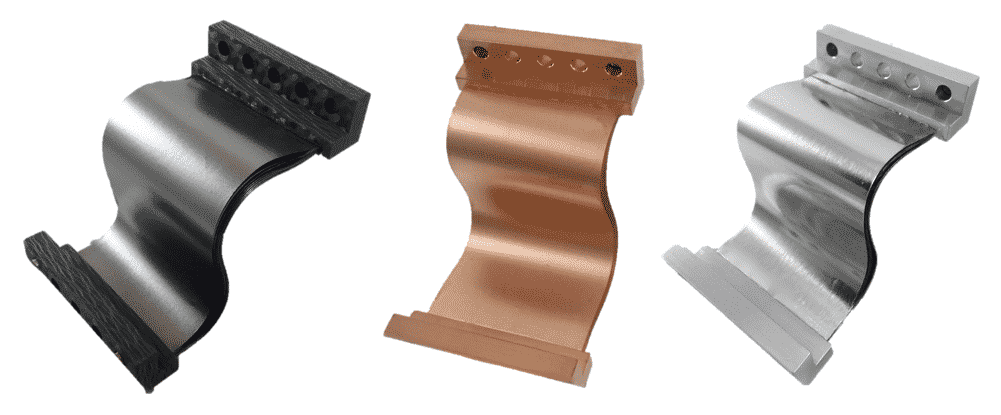
\includegraphics[width=\textwidth]{thermal_straps_commercial.png}
  \caption{Kommerziell erhältliche Wärmeleitbänder aus \ac{pgs} (links), Kupfer und Aluminium~\cite{Thermal-Straps}}\label{fig:thermalstraps_commercial}
\end{figure}

\definecolor{good}{RGB}{200,255,200}   % hellgrün
\definecolor{medium}{RGB}{255,255,200} % hellgelb
\definecolor{bad}{RGB}{255,200,200}    % hellrot

\begin{table}
  \centering
  \caption{Ampelbewertung von Materialien für Wärmeleitbänder.}\label{tab:strap_materials}

  % 1. Spalte als Box-Spalte, damit \\ innerhalb der ZELLE umbricht
  \begin{tabular}{>{\raggedright\arraybackslash}m{3cm} m{3.2cm} m{3.2cm} m{3cm}}
    \toprule[1pt]
    Eigenschaft & Kupfer\cite{Thermtest-DB} & Aluminium\cite{Thermtest-DB} & PGS \nobreak{(Graphit)}\cite{HPMS-PGS} \\
    \midrule[0.5pt]

    \makecell[l]{Wärmeleit-\\fähigkeit\\in Ebene}
      & \cellcolor{medium}\SI{397.48}{\watt\per\meter\per\kelvin}
      & \cellcolor{bad}\SI{225.94}{\watt\per\meter\per\kelvin}
      & \cellcolor{good}\SIrange{1050}{1800}{\watt\per\meter\per\kelvin} \\

    \makecell[l]{Wärmeleit-\\fähigkeit\\durch Ebene}
      & \cellcolor{good}\SI{397.48}{\watt\per\meter\per\kelvin}
      & \cellcolor{medium}\SI{225.94}{\watt\per\meter\per\kelvin}
      & \cellcolor{bad}\SIrange{10}{26}{\watt\per\meter\per\kelvin} \\

    Dichte
      & \cellcolor{bad}\SI{8940}{\kilogram\per\cubic\meter}
      & \cellcolor{medium}\SI{2698}{\kilogram\per\cubic\meter}
      & \cellcolor{good}\SIrange{1500}{2100}{\kilogram\per\cubic\meter} \\

    Elektrische \makecell[l]{\\Isolation}
      & \cellcolor{bad}Schlecht
      & \cellcolor{bad}Schlecht
      & \cellcolor{bad}Schlecht \\
    \bottomrule[1pt]
  \end{tabular}
\end{table}

Aufgrund der höchsten Wärmeleitfähigkeit in der Ebene vom \ac{pgs} HGS-012 der Firma HPMS Graphite~\cite{HPMS-PGS} wurde dieses ausgewählte.
Um ein verwendbares Wärmeleitband zu konstruieren, soll dieses aus 32 Schichten bestehen, \SI{4}{\centi\meter} breit und 
\SI{10}{\centi\meter} lang sein, wodurch es ermöglicht werden soll, dass die Heatpipe keine Biegungen hat.
Die Anbindungen bzw. Endstücke der Wärmeleitbänder, sowie Kontaktwiederstände durch Klebstoffe oder ähnliche Verbindungsmethoden werden ignoriert.
Der Wärmeleitwiederstand ergibt sich durch einsetzen von Gleichung \ref{eq:fourier_1d} in \ref{eq:waermewiederstand}:

\begin{equation*}
  R_\mathrm{Wärmeleitband} = \frac{\Delta x}{\lambda A}
\end{equation*}

Mit $\Delta x = \SI{10}{\centi\meter}$, $\lambda = \SI{1800}{\watt\per\meter\kelvin}$ und $A = 32 \cdot \SI{0,012}{\milli\meter} \cdot \SI{4}{\centi\meter} = \SI{15,36}{\milli\meter\squared}$
ergibt sich $R_\mathrm{Wärmeleitband} = \SI{3,617}{\kelvin\per\watt}$

\subsection{Gesamte Schnittstelle}\label{sec:gesamte_schnittstelle}

Mittels einer Kombination von \ac{pgs} und Heatpipe kann eine Wärmebrücke gebildet werden, die den Wärmeleitwiederstand
minimiert. Eine Schematische Darstellung der Thermalen Schnittstelle ist in Abbildung~\ref{fig:thermale_schnittstelle} zu sehen.

Wenn angenommen wird, dass die Avionik aus vier separaten \ac{pcb} mit einer Gesamtleistung von \SI{40}{\watt}~(\ref{tab:avionik_leistung}) besteht, müssen pro Wärmeleitband \SI{10}{\watt} übertragen werden.
Dabei entsteht nach Gleichung~\ref{eq:waermewiederstand} eine Temperaturerhöhung über das Wärmeleitband von $\SI{10}{\watt} \cdot \SI{3,617}{\watt\per\kelvin} = \Delta T_\mathrm{Wärmeleitband} = \SI{36,17}{\kelvin}$.
Die Heatpipe überträgt den vollständigen Wärmestrom und hat eine Temperaturerhöhung von $\SI{40}{\watt} \cdot \SI{0,3}{\watt\per\kelvin} = \Delta T_\mathrm{Heatpipe} = \SI{12}{\kelvin}$.

Von der Quelle bis zur Senke ergibt sich also ein Temperaturgradient von $\Delta T_\mathrm{Heatpipe} + \Delta T_\mathrm{Wärmeleitband} = \Delta T_\mathrm{ges} = \SI{48,17}{\kelvin}$.
Eine Schematische Darstellung der Schnittstelle sieht man in Abbildung~\ref{fig:thermale_schnittstelle}. Für die Nötige Temperatur an der Senke
erhält man $T_\mathrm{Senke} = T_C - \Delta T_\mathrm{ges} = \SI{314,13}{\kelvin}$. Die Masse der Schnittstelle wird nicht berücksichtigt, da diese
unabhängig von der Kühlung an der Senke notwendig ist und sich auf wenige Gramm beschränkt.

\begin{figure}
  \centering
  \begin{tikzpicture}
    \node at (0,0) [style={single arrow, draw}, minimum height=0.5cm, minimum width=1.5cm, shape border rotate=90, thick]{$\dot{Q}$}; % Wärmestrom pfeil

    \draw[thick] (0,-1) -- (0,-3.1);

    \draw[thick] (0,-3.1) -- (-0.2,-3.2); % heatpipe resistor
    \draw[thick] (-0.2,-3.2) -- (0.2,-3.4);
    \draw[thick] (0.2,-3.4) -- (-0.2,-3.6);
    \draw[thick] (-0.2,-3.6) -- (0.2,-3.8);
    \draw[thick] (0.2,-3.8) -- (-0.2,-4);
    \draw[thick] (-0.2,-4) -- (0.2,-4.2);
    \draw[thick] (0.2,-4.2) -- (0,-4.3);

    \node[rotate=90] at (-0.5,-3.7) {Heatpipe};
    \node at (2.5,-3.7) {$R_{\mathrm{Heatpipe}} = \SI{0,3}{\kelvin\per\watt}$};

    \draw[thick] (0,-4.3) -- (0,-6.4);

    \draw[thick] (0,-6.4) -- (2.1,-6.4);

    \fill (0,-6.4) circle (1.5pt); %knotenpunkt

    \begin{scope}[shift={(-1,-6.4)}, rotate=90]
      \draw[thick] (0,-3.1) -- (-0.2,-3.2); % thermal strap resistor
      \draw[thick] (-0.2,-3.2) -- (0.2,-3.4);
      \draw[thick] (0.2,-3.4) -- (-0.2,-3.6);
      \draw[thick] (-0.2,-3.6) -- (0.2,-3.8);
      \draw[thick] (0.2,-3.8) -- (-0.2,-4);
      \draw[thick] (-0.2,-4) -- (0.2,-4.2);
      \draw[thick] (0.2,-4.2) -- (0,-4.3);
    \end{scope}


    \node at (2.7,-5.9) {Wärmeleitband};
    \node at (2.7,-6.9) {$R_{\mathrm{Wärmeleitband}} = \SI{3,617}{\kelvin\per\watt}$};

    \draw[thick] (3.3,-6.4) -- (5.4,-6.4);

    \node at (6.4,-6.4) [style={single arrow, draw}, minimum height=0.5cm, minimum width=1.5cm, shape border rotate=180, thick]{$\frac{\dot{Q}}{4}$}; % Wärmestrom pfeil

    \draw[thick] (0,-6.4) -- (0,-8.4);

    \draw[thick] (0,-8.4) -- (2.1,-8.4);

    \fill (0,-8.4) circle (1.5pt);% knotenpunkt 2

    \begin{scope}[shift={(-1,-8.4)}, rotate=90]
      \draw[thick] (0,-3.1) -- (-0.2,-3.2); % thermal strap resistor 2
      \draw[thick] (-0.2,-3.2) -- (0.2,-3.4);
      \draw[thick] (0.2,-3.4) -- (-0.2,-3.6);
      \draw[thick] (-0.2,-3.6) -- (0.2,-3.8);
      \draw[thick] (0.2,-3.8) -- (-0.2,-4);
      \draw[thick] (-0.2,-4) -- (0.2,-4.2);
      \draw[thick] (0.2,-4.2) -- (0,-4.3);
    \end{scope}

    \node at (2.7,-7.9) {Wärmeleitband};
    \node at (2.7,-8.9) {$R_{\mathrm{Wärmeleitband}} = \SI{3,617}{\kelvin\per\watt}$};

    \draw[thick] (3.3,-8.4) -- (5.4,-8.4);

    \node at (6.4,-8.4) [style={single arrow, draw}, minimum height=0.5cm, minimum width=1.5cm, shape border rotate=180, thick]{$\frac{\dot{Q}}{4}$}; % Wärmestrom pfeil

    \draw[thick] (0,-8.4) -- (0,-9);

    \node[rotate=90] at (0,-9.5) {$\cdots$};

    \draw[->, thick, -{Stealth[length=0.25cm]}] (-1.5,-6) -- node [pos=0,above=1pt] {$g$} (-1.5,-8); % Gravitation
  \end{tikzpicture}
  \caption{\ac{rom} der Thermalen Schnittstelle aus Heatpipe und Wärmeleitbändern. Hier sind nur 2 von 4 Wärmeleitbändern dargestellt.}\label{fig:thermale_schnittstelle}
\end{figure}

\section{PCM}\label{sec:pcm}

Nutzung eines \ac{pcm} mit Fest-Flüssig Übergang ist eine weit verbreitete Lösung in der Luft- und Raumfahrtindustrie um für begrenzte Zeiträume Elektronik in einem akzeptablen
Temperaturbereich zu halten. Auch wenn \ac{pcm} Lösungen generell eine hohe Masse haben, wird das oft aufgrund der ansonsten idealen Eigenschaften inkauf genommen:
Durch die hohe spezifische Schmelzenthalpie, kann rein passiv eine große Wärmemenge, bei einem isothermen Prozess, absorbiert werden. Aufgrund dessen
kann ein von der Umwelt isoliertes \ac{atm} entwickelt werden, das nicht mit stark schwankenden Zuständen der Sonneneinstrahlung und Lufttemperatur
zurecht kommen muss. Auch wenn ein \ac{pcm} mit Flüssig-Gas Übergang meist eine etwa 10-fach höhere Verdampfungsenthalpie hat, wird diese Art
generell nicht verwendet, da der Dichteunterschied zwischen Flüssig- und Gasphase zu extremen Drücken führen würden, falls Wiederverwendbarkeit
verlangt wird und somit ein Druckkörper nötig ist. Alternativ kann die Gasphase auch aus dem Fahrzeug abgelassen werden in einem Prozess der
Vapour Venting genannt wird. Hierbei geht jedoch die Wiederverwendbarkeit verloren, da vor jedem Start die Flüssigphase neu getankt werden muss.
Weiter kann das Vapour Venting trotz der geringen Massenströme zu Momenten führen, die das Fahrzeug destabilisieren; besonders im Überschallbereich
können unintuitive Kräfte durch Interaktionen mit dem Überschallstrom entstehen~\cite{Deere-2011}, die aufwendige \ac{cfd}-Simulationen oder Tests benötigen.
Dementsprechend wird nur ein Fest-Flüssig \ac{pcm} analysiert.

Für die Auswahl eines geeigneten \ac{pcm} sind spezifische Schmelzenthalpie und Schmelztemperatur entscheidend.
Die Wärmeleitfähigkeit ist zwar auch sehr relevant, ist jedoch für alle Materialien zu schlecht und muss durch Lamellen oder ähnliche Wärmetauschende Strukturen verbessert werden,
wobei dabei \ac{pcm} Masse mit Strukturmasse ersetzt wird und somit die Wärmekapazität sinkt. Das Volumen der Wärmeleitenden Struktur welches
\ac{pcm} ersetzt wird Void Fraction genannt, da es gewissermaßen eine Leerstelle im \ac{pcm} bildet, die wie gesagt keine latente Wärmeaufnahme hat. Hier
wird ein Void Fraction von $F = 0.1$ gewählt. Eine Optimierung der Lamellenstruktur kann bei gleich bleibender Masse in einer erhöhten
Wärmeleitfähigkeit resultieren, was jedoch in dieser Arbeit nicht durchgeführt wird. Abbildung~\ref{fig:pcm_struktur} zeigt ein Drahtmodell der Struktur,
welche eine einfache Box ist die für Länge und Breite die selbe Dimension hat und weiter in Höhe variieren kann. In der Box ist
das \ac{pcm} zwischen parallelen Lamellen vorhanden.

\begin{table}
  \centering
  \caption{Ampelbewertung für Alkane als \ac{pcm} \cite{NIST}.}\label{tab:pcm_auswahl}
  \label{tab:pcm_alkane_nist}
  \begin{tabular}{>{\raggedright\arraybackslash}m{3.1cm} m{3.1cm} m{3.1cm} m{3.1cm}}
    \toprule[1pt]
    Eigenschaft & n-Hexadecan & n-Octadecan & n-Eicosan \\
    \midrule[0.5pt]

    Schmelzpunkt
      & \cellcolor{bad}\SI{291}{\kelvin}
      & \cellcolor{medium}\SI{301}{\kelvin}
      & \cellcolor{good}\SI{310}{\kelvin} \\

    Schmelzenthalpie
      & \cellcolor{bad}\SI{230400}{\joule\per\kilo\gram}
      & \cellcolor{medium}\SI{239300}{\joule\per\kilo\gram}
      & \cellcolor{good}\SI{240999}{\joule\per\kilo\gram} \\
    \bottomrule[1pt]
  \end{tabular}
\end{table}

Die Tabelle~\ref{tab:pcm_auswahl} zeigt die drei gängigsten Organischen Alkane, welche als \ac{pcm} verwendet werden im Vergleich.
Demnach hat n-Eicosan die besten Eigenschaften, mit insbesondere einem perfekten Schmelzpunkt kurz unter den \SI{314,13}{\kelvin} der Senke,
wie in Kapitel~\ref{sec:thermale_schnittstelle} berechnet.
Um die Masse und latente Wärmekapazität des \ac{pcm} zu berechnen wurde das in \ref{lst:pcm_python_pseudo} dargestellte Python-Programm verwendet.
Das \ac{pcm} wird dort als isobar und isotherm angenommen und hat eine unendliche Wärmeleitfähigkeit. Des weiteren befindet es sich
in einer Aluminium-Box mit \SI{1}{\milli\meter} Wanddicke und einem der Void Fraction entsprechenden internen Volumenanteil an  Aluminium von $F = 0.1$.
Die Dimensionen der Breite und Tiefe der Box wurden gleich gesetzt; die Höhe der Box bildet die zweite Variable.
Anschließend werden mit der Funktionen \texttt{total\_mass} die Masse und \texttt{total\_heat} die latente Wärmekapazität durch Bilanzierung
der Gleichung~\ref{eq:latente_waerme} berechnet.
Kapazitäts- und Massenkonturen abhängig von Seitenlänge und Höhe können in Abbildung~\ref{fig:pcm_waermestrom_vorauslegung} gesehen werden.

Bei einer Flugdauer von \SI{1200}{\second} und einem Wärmestrom von \SI{40}{\watt} ergibt sich eine nötige latente Wärmekapazität von
\SI{48000}{\joule}, eine Seitenlänge der Aluminium-Box von \SI{6,749}{\centi\meter} und eine Gesamtmasse von \SI{346,610}{\gram}.
Da ein Würfel von allen Quadern das größte Volumen-Oberflächenverhältnis hat, sind alle Kanten gleich lang.

\begin{lstlisting}[float, language=Python, caption={Berechnung der Masse und Latenten Wärmekapazität des \ac{pcm} in der pcm.py}, label={lst:pcm_python_pseudo}]
rho_alu = 2700     # aluminium density [kg*m^-3]
rho_pcm = 788      # pcm density [kg*m^-3]
h       = 240998.9 # pcm latent heat [J*kg^-1]
F       = 0.1      # void fraction
t       = 0.001    # wall thickness [m]

def total_mass(L, H): # pcm mass including case and fins
    return (rho_alu * (L**2 * H - (L - 2*t)**2 * (H - 2*t))
            + (F * rho_alu + (1 - F) * rho_pcm) * (L - 2*t)**2 * (H - 2*t)) 

def total_heat(L, H): # pcm latent heat capacity
    #...#
    pcm_heat  = (1 - F) * rho_pcm * (L - 2*t)**2 * (H - 2*t) * h
    return pcm_heat
\end{lstlisting}

\section{Radiator}\label{sec:Radiator}

Bei Radiatoren ist ein hoher Emissions- und niedriger Absorptionsgrad nach Gleichung~\ref{eq:radiation} dimensionierend, da die Temperatur den Anforderungen nach limitiert ist
und die Fläche minimiert werden muss, weil diese proportional zu eingehenden Wärmeströmen aus der Umgebung ist, wie etwa die Sonneneinstrahlung oder die Luft, welche auch möglichst gering gehalten werden sollen.
\\
Als Beschichtung wurde AZ-93 der Firma AZ Technology LLC.~\cite{AZ-Technology} ausgewählt. Dabei handelt es sich um eine in der Raumfahrt
weit verbreitete inorganische Farbe mit günstigen Eigenschaften, welche Tabelle \ref{tab:az-93_eigenschaften} entnommen werden können.
Abbildung~\ref{fig:radiator_flaeche_leistung} ist eine Visualisierung der Gleichung~\ref{eq:radiation} und zeigt Leistungskonturen eines
Radiators mit den Eigenschaften aus Tabelle~\ref{tab:az-93_eigenschaften} je nach Fläche und Temperatur.

\begin{table}

  \centering
  \caption{AZ-93 Spezifikationen~\cite{AZ-Technology}}\label{tab:az-93_eigenschaften}

  \begin{tabular}{ll}

    \toprule[1pt]
    $\varepsilon_{\text{t}}$ & $0.91 \pm 0.02$ \\

    \midrule[0.5pt]
    $\alpha_{\text{s}}$ & $0.15 \pm 0.02$ \\

    \midrule[0.5pt]
    Temperaturbereich  & \SI{-180}{\degreeCelsius} bis \SI{1400}{\degreeCelsius} \\

    \bottomrule[1pt]
  \end{tabular}
\end{table}

Für eine rein radiative Kühlung der Avionik ergibt sich für \SI{40}{\watt} der Avionik und einen spezifischen Wärmestrom der Sonne (Solarer Wärmestrom) von \SI{1}{\kilo\watt\per\meter\squared}
bei einem \SI{50}{\percent} Dutycycle, durch die Rotation der Rakete bzw. der Schattierung des halben Radiators durch die Rakete selbst auf der Sonnenabgewandten Seite, den Eigenschaften aus
\ref{tab:az-93_eigenschaften} und einer Temperatur von $T_\mathrm{senke} = \SI{314,13}{\kelvin}$
nach eine Fläche von \SI{996,163}{\centi\meter\squared}.
Der Solare Wärmestrom wurde für \SI{1}{\meter} über dem Meeresspiegel bei der Sommersonnenwende in Campo Militar de Santa Margarida beim höchsten Sonnenstand
mittels des Online-Tools www.sonnenverlauf.de berechnet, da dort die Demonstrator-Rakete von \ac{blast} starten wird und als Richtwert für \ac{blast} verwendet werden kann.
Die Radiatorleistung ergibt sich demnach zu $\dot{Q}_\mathrm{Radiator} = \SI{47.471}{\watt}$.
In \ref{lst:setup_json} und \ref{lst:radiator_python_pseudo} ist der Programmcode der zur Berechnung verwendet wurde zu sehen.

\begin{lstlisting}[float, language=python, caption={Setup Werte aus der setup.json}, label={lst:setup_json}]
  {
    #...#
    "avionics_power": 40,
    "target_temperature": 36.85,
    "emittance": 0.91,
    "absorptance": 0.15,
    "solar_flux": 1000,
  }
\end{lstlisting}

\begin{lstlisting}[float, language=Python, caption={Berechnung der Radiatorfläche in der radiator.py}, label={lst:radiator_python_pseudo}]
  #...#
  avionics_power = data["avionics_power"]
  e = data["emittance"]
  a = data["absorptance"]
  solar_flux = data["solar_flux"]
  target_temperature = data["target_temperature"]

  def radiator_area(avionics_power, target_temperature, e, a, solar_flux): # radiator area
    return (avionics_power / (e * Stefan_Boltzmann * target_temperature**4 - 0.5 * solar_flux * a))
\end{lstlisting}

\section{PCM-Radiator-Hybrid}\label{sec:pcm_radiator_hybrid}

Eine Hybridlösung wird auch in Erwägung gezogen, um die Masse durch Nutzung eines Radiators zu minimieren, wobei wegen aerodynamischer Aufheizung für kurze Zeit ein PCM gebraucht werden könnte.
Für die Vorauslegung wird die Außenkontur der Rakete von Spitze bis Avionik-Sektion, mit Hilfe der Nußelt-Beziehungen, als Längsangeströmte ebene Platte angesehen,
wie in Abbildung~\ref{fig:rakete_kontour_zeichnung} dargestellt ist.
Um zu wissen, ob hier die Beziehung für laminare oder turbulente Grenzschichten angewandt werden soll, müssen zunächst die Gültigkeitsbereiche der Reynolds- und Prandtlzahl (\ref{eq:prandtl},~\ref{eq:reynolds}) überprüft werden.
Mittels der Nußelt-Beziehung wird der Wärmeübergangskoeffizient $\alpha$ bestimmt und dann in Gleichung~\ref{eq:qdot_recovery} eingesetzt, um auf den spezifischen Wärmestrom zu schließen.

Die Außenstruktur der Rakete besteht aus dem zylindrischen Hüllensegment und einem von-Kármán-Nasenprofil das eine
Spezialform der Haack Serie ist \cite{Stoney-1954}. Die analytische Beschreibung lautet:

\begin{equation*}
  \label{eq:karman_nase}
  x(t) = \frac{R}{\sqrt{\pi}} \cdot \sqrt{
  \cos^{-1}\left(1 - \frac{2t}{L} \right)
  - \frac{1}{2} \cdot \sin\left(2 \cdot \cos^{-1}\left(1 - \frac{2t}{L} \right) \right)
  }
  \quad \text{für } t \in [0, L]
\end{equation*}

Hierbei ist $x(t)$ der Radiusverlauf des rotationssymmetrischen Nasenprofils entlang der Längskoordinate $t$, beginnend an der Spitze $(t=0)$ bis zur Basis $(t=L)$.
Die Gesamtlänge der Nase ist $L = \SI{1250}{\milli\meter}$. Der maximale Radius an der Basis beträgt $R = \SI{125}{\milli\meter}$, und entspricht dem Gesamtdurchmesser der Rakete von $D = \SI{250}{\milli\meter}$.

Die Funktion der Nase wurde mithilfe von einem \ac{cad} Programm skizziert und die Konturlänge zu \SI{1,01}{\meter} vermessen. Wenn der Radiator über den vollständigen Umfang der Rakete
bei einem Durchmesser von $D = \SI{250}{\milli\meter}$ modelliert wird, ist der Radiator eine \SI{12,684}{\centi\meter} lange Sektion.
Daraus folgt eine Konturlänge von \SI{1,074}{\meter} bis zum Mittelpunkt des Radiators, an der Stelle alle lokalen Größen berechnet wurden.

\begin{figure}
  \centering
  \begin{tikzpicture}[rotate border/.style={shape border uses incircle, shape border rotate=#1}, scale=0.8]
    \draw[thick] (3,3) -- (3,-1) -- (9,-1) -- (9,3);
    \draw[thick] (3,3) -- node [midway, above] {Avionik Sektion}  (9,3);
    \draw[thick] (4,3) -- (4,-1); % PCM Lamellen
    \draw[thick] (3,-0.5) -- (4,-0.5);
    \draw[thick] (3,0) -- (4,0);
    \draw[thick] (3,0.5) -- (4,0.5);
    \draw[thick] (3,1) -- (4,1);
    \draw[thick] (3,1.5) -- (4,1.5);
    \draw[thick] (3,2) -- (4,2);
    \draw[thick] (3,2.5) -- (4,2.5);
    \node at (-0.5,2) [style={single arrow, draw}, minimum height=3cm, minimum width=0.5cm, thick]{$\dot{Q}_{\mathrm{Umwelt}}$}; % Wärmestrom pfeil
    \node at (-0.5,0) [style={single arrow, draw}, minimum height=4.5cm, minimum width=1.5cm, shape border rotate=180, thick]{$\dot{Q}_{\mathrm{Radiator}}$}; % Wärmestrom pfeil
    \node at (6.5,1)[style={single arrow, draw}, minimum height=3cm, minimum width=0.5cm, shape border rotate=180, thick]{$\dot{Q}_{\mathrm{Avionik}}$}; % Wärmestrom pfeil
    \draw[->, thick, -{Stealth[length=0.25cm]}] (1,3.75) node [above=1pt] {PCM mit Lamellen} -- (3.5,2.6);
  \end{tikzpicture}
  \caption{PCM Wärmestrom ohne aerodynamische Aufheizung}\label{fig:pcm_waermestrom_diagramm}
\end{figure}

In Abbildung~\ref{fig:pcm_waermestrom_diagramm} sieht man eine Schematische Darstellung der Konstruktion und speziell die Wärmeströme
für den Fall, dass das System am Solidus-Punkt im Gleichgewicht steht. Hingegen kann man in Abbildung~\ref{fig:pcm_waermestrom_aufheizung_diagramm}
den Zustand sehen, in dem der Umweltwärmestrom durch aerodynamische Aufheizung gestiegen ist und somit das \ac{pcm} anfängt zu schmelzen.
Wegen des \ac{pcm} und der Annahme, dass alle Wärmeleitkoeffizienten unendliche groß sind, wird das System als isotherm modelliert und die Avionik-Sektion als
adiabat.

\begin{figure}
  \centering
  \begin{tikzpicture}[rotate border/.style={shape border uses incircle, shape border rotate=#1}, scale=0.8]
    \draw[thick] (3,3) -- (3,-1) -- (9,-1) -- (9,3);
    \draw[thick] (3,3) -- node [midway, above] {Avionik Sektion}  (9,3);
    \draw[thick] (4,3) -- (4,-1); % PCM lamellen
    \draw[thick] (3,-0.5) -- (4,-0.5);
    \draw[thick] (3,0) -- (4,0);
    \draw[thick] (3,0.5) -- (4,0.5);
    \draw[thick] (3,1) -- (4,1);
    \draw[thick] (3,1.5) -- (4,1.5);
    \draw[thick] (3,2) -- (4,2);
    \draw[thick] (3,2.5) -- (4,2.5);
    \node at (-0.5,2) [style={single arrow, draw}, minimum height=4.5cm, minimum width=1.5cm, thick]{$\dot{Q}_{\mathrm{Umgebung}}$}; % Wärmestrom pfeil
    \node at (-0.5,0) [style={single arrow, draw}, minimum height=4.5cm, minimum width=1.5cm, shape border rotate=180, thick]{$\dot{Q}_{\mathrm{Radiator}}$}; % Wärmestrom pfeil
    \node at (6.5,1)[style={single arrow, draw}, minimum height=3cm, minimum width=0.5cm, shape border rotate=180, thick]{$\dot{Q}_{\mathrm{Avionik}}$}; % Wärmestrom pfeil
  \end{tikzpicture}
  \caption{PCM Wärmestrom bei aerodynamischer Aufheizung}\label{fig:pcm_waermestrom_aufheizung_diagramm}
\end{figure}

\begin{figure}
  \centering
  \begin{tikzpicture}
    \draw[thick] (0,0) arc [start angle=90, end angle=270, x radius=5cm, y radius= 1.5cm]; %nosecone
    \draw[thick] (0,0) -- (3,0); % hülle
    \draw[thick] (0,-3) -- (3,-3); % hülle
    \draw[thick] (-5.75,-1.5) -- (-5.25,-1.5); % maß links
    \draw[thick] (1,0.25) -- (1,0.75); % maß rechts
    \draw[thick] (0,0.5) arc [start angle=90, end angle=180, x radius=5.5cm, y radius= 2cm]; % maß bogen
    \draw[thick] (0,0.5) -- node [near start, above] {Konturlänge} (1,0.5); % maß grade sektion
    \draw[->, thick, -{Stealth[length=0.25cm]}] (-10,0.5) -- node [midway, above] {Luftstrom} (-7,0.5); % free stream pfeile
    \draw[->, thick, -{Stealth[length=0.25cm]}] (-10,-0.5) -- (-7,-0.5); % Strompfeile
    \draw[->, thick, -{Stealth[length=0.25cm]}] (-10,-1.5) -- (-7,-1.5);
    \draw[->, thick, -{Stealth[length=0.25cm]}] (-10,-2.5) -- (-7,-2.5);
    \draw[->, thick, -{Stealth[length=0.25cm]}] (-10,-3.5) -- (-7,-3.5);
    \draw[thick] (0,0) -- (0,-2.5); % casing wall
    \draw[thick] (2,0) -- (2,-2.5); % casing wall
    \draw[thick] (0,-2.5) -- (2,-2.5); % casing bottom
    \node at (1,-1.5) [style={single arrow, draw}, minimum height=0.5cm, minimum width=1.5cm, rotate=90, thick]{$\dot{Q}_{\mathrm{Avionik}}$}; % Wärmestrom pfeil
  \end{tikzpicture}
  \caption{Konturlänge vom Staupunkt der Rakete bis zum Mittelpunkt des Radiators}\label{fig:rakete_kontour_zeichnung}
\end{figure}


Die Software zur Berechnung aller Bilanzgleichungen für Dimensionen und Massen besteht aus einer Reihe an Python Programmen und Datenstrukturen.
Das Hauptprogramm \texttt{main.py} ruft alle Unterprogramme in der richtigen Reihenfolge: zuerst die \texttt{radiator.py} zur Berechnung
der Radiator Dimension mithilfe der Randbedingungen aus der \texttt{setup.json}, danach wird die \texttt{hybrid.py} (\ref{lst:hybrid_python_pseudocode}) aufgerufen um die Aerodynamischen Wärmeströme
mittels der Nußelt-Beziehung zu bestimmen, anschließend werden die Ergebnisse in die \texttt{pcm.py} geladen, um abhängig von der Radiatorfläche
und den Wärmeströmen die Kapazität und Masse des \ac{pcm} zu bestimmen.
In Abbildung~\ref{fig:dimensionierung_ablauf} sieht man schematisch wie die Dimensionierung in der Software abläuft.

\begin{figure}
  \centering
  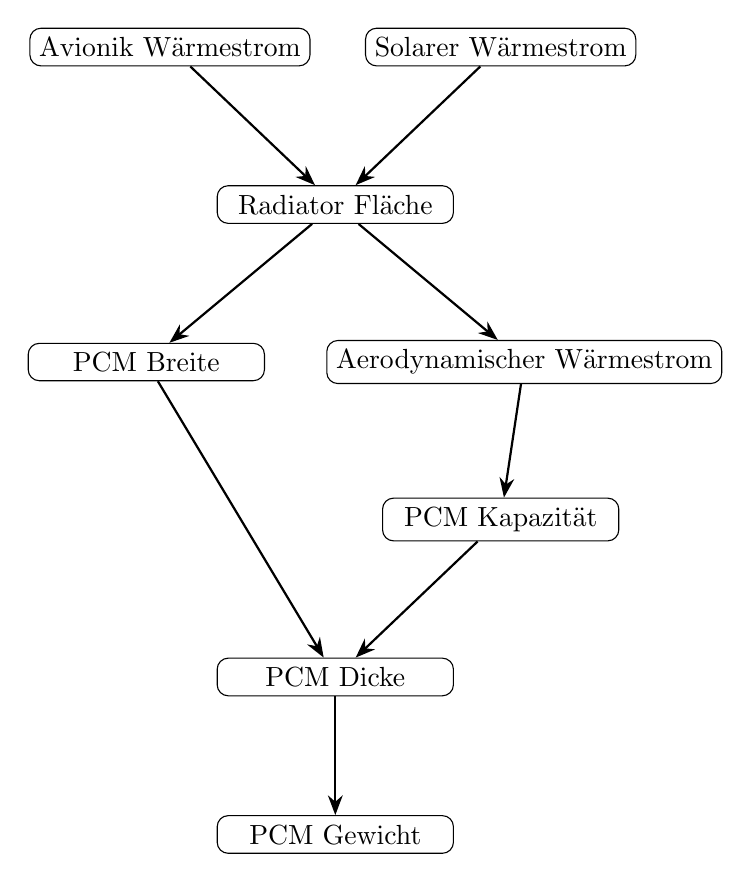
\begin{tikzpicture}[
    sibling distance=10em,
    every node/.style = {
      shape=rectangle,
      rounded corners,
      draw,
      align=center,
      minimum width=3cm
    },
    edge from parent/.style = {
      draw,
      ->,
      -{Stealth[length=0.25cm]},
      thick
    },
    arrow/.style = {
      ->,
      -{Stealth[length=0.25cm]},
      thick
    }
  ]

    % Top nodes
    \node (avionik) at (-2.1, 4) {Avionik Wärmestrom};
    \node (sonne)   at ( 2.1, 4) {Solarer Wärmestrom};

    % Radiator Fläche centered below
    \node (radiator) at (0, 2) {Radiator Fläche};

    % Children of Radiator
    \node (breite) at (-2.4, 0) {PCM Breite};
    \node (aerodynamisch) at (2.4, 0) {Aerodynamischer Wärmestrom};

    % PCM Kapazität as a separate node (not a child directly)
    \node (kapazitaet) at (2.1, -2) {PCM Kapazität};

    % PCM Höhe node below the center of breite and kapazitaet
    \node (hoehe) at (0, -4) {PCM Dicke};
    \node (gewicht) at (0, -6) {PCM Gewicht};

    % Arrows
    \draw[arrow] (avionik) -- (radiator);
    \draw[arrow] (sonne) -- (radiator);
    \draw[arrow] (radiator) -- (breite);
    \draw[arrow] (radiator) -- (aerodynamisch);
    \draw[arrow] (aerodynamisch) -- (kapazitaet);
    \draw[arrow] (breite) -- (hoehe);
    \draw[arrow] (kapazitaet) -- (hoehe);
    \draw[arrow] (hoehe) -- (gewicht);

  \end{tikzpicture}
  \caption{Ablauf der Dimensionierung in der Vorauslegungs-Software. Pfeile stellen Abhängigkeiten dar.}\label{fig:dimensionierung_ablauf}
\end{figure}

Wie in Abbildung~\ref{fig:re_pr_flugsimulation} dargestellt, liegt die Prandtl-Zahl im Gültigkeitsbereich sowohl für die turbulente als auch
für die laminare Grenzschicht. Die Reynolds-Zahl überschreitet jedoch zeitweise mit Werten bis zu \SI{2.4e7} die Gültigkeitsbereiche.
Aufgrund fehlender alternativer analytischer Methoden wurde dennoch die Nußelt-Beziehung nach Gleichung~\ref{eq:nusselt_turbulent} für turbulente Grenzschichten angewendet.

\begin{figure}
  \centering
  \includegraphics[width=\linewidth]{../../Code/re_pr_during_flight.pdf}
  \caption{Reynolds- und Prandtlzahl während kritischer Phase im Flug}\label{fig:re_pr_flugsimulation}
\end{figure}

Das Ergebnis der Berechnung ist in Abbildung~\ref{fig:pcm_waermestrom_vorauslegung} zu sehen, mit der Radiatorleistung $\dot{Q}_\mathrm{Radiator} = \SI{47.471}{\watt}$
aus Kapitel~\ref{sec:Radiator} und dem Wärmestrom aus der Umwelt $\dot{Q}_\mathrm{Umwelt}$, der aus Sonneneinstrahlung wie in \ref{sec:Radiator} modelliert
und der aerodynamischen Aufheizung besteht.
Der Wärmestrom $\dot{Q}_\mathrm{Rein}$ ist die Summe aus Avionik Wärmestrom $\dot{Q}_\mathrm{Avionik}$ und dem Umwelt Wärmestrom $\dot{Q}_\mathrm{Umwelt}$.

\begin{figure}[H]
  \centering
  \includegraphics[width=\linewidth]{../../Code/pcm_radiator_hybrid_heatflux_nosim.pdf}
  \caption{PCM Wärmeströme während dem Flug}\label{fig:pcm_waermestrom_vorauslegung}
\end{figure}

Erkennbar ist, dass mit bis zu \SI{20}{\kilo\watt} ein extrem hoher Wärmestrom durch die aerodynamisch Aufheizung entsteht.
Auch wenn dieser nur etwa \SI{100}{\second} andauert, ist er ausreichend um die notwendige Masse des \ac{pcm} (inklusive der Aluminium Struktur)
auf \SI{4,256}{\kilo\gram} zu erhöhen. Abgesehen von der höheren notwendigen latenten Wärmekapazität von \SI{626817.571}{\joule} führen auch zusätzlich geometrische
Verluste zu der erhöhten Masse, da das Aspektverhältnis aufgrund der Einschränkung durch die Radiatorfläche weit von der idealen Würfelform entfernt ist.

% ----------- Diskussion & Schlussfolgerungen----------------------------------------
\newpage
\chapter{Simulation}\label{chap:Simulation}

\section{CFD}\label{sec:sim_cfd}

\begin{figure}[H]
    \centering
    \begin{subfigure}[t]{0.7\textwidth}
        \centering
        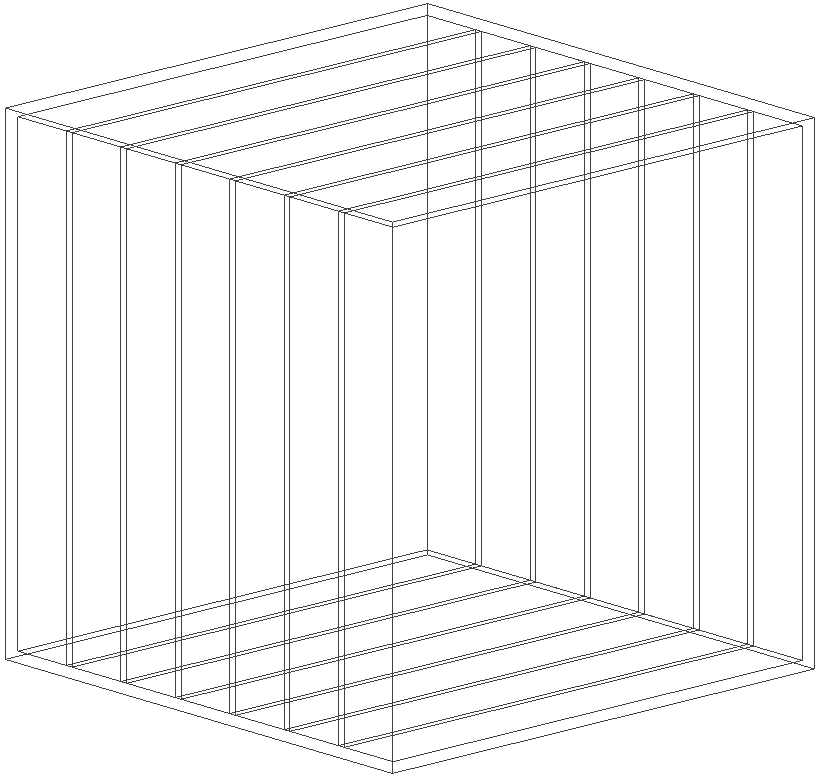
\includegraphics[height=9cm]{ansyspost/pcm/40WPCM_struktur.png}
        \caption{\ac{pcm} Struktur}\label{fig:pcm_struktur}
    \end{subfigure}
    \hfill
    \begin{subfigure}[t]{0.15\textwidth}
        \centering
        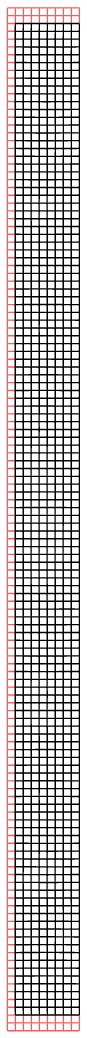
\includegraphics[height=9cm]{ansyspost/pcm/2DPCM_mesh.png}
        \caption{\ac{pcm} Mesh}\label{fig:pcm_mesh}
    \end{subfigure}
    \caption{\ac{pcm} Struktur und vereinfachtes Mesh}\label{fig:pcm_geometrien}
\end{figure}

Die Vorauslegungwurde mit folgenden Werten durchgeführt:\\
- Isotherm auf: \SI{38}{\celsius}\\
- Avionik Abwärme: \SI{40}{W}\\
- \SI{1}{m} Kontourlänge\\
- Radiator Emissionsgrad: \SI{0,91}{} (AZ-93)\\
- Radiator Absorptionsgrad: \SI{0,15}{} (AZ-93)\\
- Icosane PCM\\
- Trajektoriensimulation\\
- \SI{1}{\kilo\watt\per\meter\squared} mit 50\% dutycycle durch Rotation der Rakete\\
Zu beachten ist, dass die Radiatorleistung konstant bleibt, da das System als isotherm mit einer
infinitesimalen Temperaturerhöhung über den Schmelzpunkt hinweg angenommen wird.\\
Als nächstes sieht man die Flugdaten




\section{Aerodynamische Aufheizung}\label{sec:sim_aerodynamisch}

Speziell für die Strömungssimulationen welche keine Koppelung mit Festkörpern haben, wurde der Density-Based Solver ausgewählt und die
Simulation als 2D Steady State durchgeführt. Das Energiemodell wurde aktiviert und für das Viskositätsmodell~\cite{Irving-2021}

Die Umströmungssimulationen der Rakete wurden an \ac{maxq} orientiert, da es als Richtwert für Aerodynamische Aufheizung genommen werden kann.
Desweiteren ist der Wert unanhängig von der Vorauslegung, wodurch Ungenauigkeiten von dort getroffenen Annahmen vermieden werden.\\


als nächstes habe ich geschaut wo der maximale dynamische Druck erreicht wurde in der Vorauslegung. Die korrespondierenden Werte des Flugzustandes
habe ich dann als Boundery Conditions in der \ac{cfd}~Simulation genommen.
Um zu verifizieren, dass dort auch die maximale Aufheizung stattfindet, habe ich 1 Sekunden vorher und nachder
im Flug die BC's auch verwendet und einen Vergleich gezogen.\\
Maximaler dynamischer Druck: 112901.25708461029 Pa at 28.691 s\\
Entsprechender Flugzustand: 10244.138 m, 750.704 m/s, -51.587°C, 254.783 hPa mit entsprechender Luft Dichte \SI{0.4006}{kg/m^3}\\
Flugzustand bei 18.691 s \ac{maxq} - $\SI{10}{\second}$: 4274.387 m, 461.355 m/s, -12.784, 594.935 hPa mit entsprechender Luft Dichte \SI{0.7960}{kg/m^3}\\
Flugzustand bei 38.691 s \ac{maxq} + $\SI{10}{\second}$: 19758.652 m, 1189.968 m/s, -56.5°C, 56.93 hPa mit entsprechender Luft Dichte \SI{0.0915}{kg/m^3}\\
Flugzustand bei 48.7 s \ac{maxq} + $\SI{20}{\second}$: 32439.616 m, 1393.377 m/s, -43.269°C, 8.136 hPa mit entsprechender Luft Dichte \SI{0.01233001}{kg/m^3}\\
Da wie in~\ref{fig:spezifischer_waermestrom_maxQ_simulationen} zu sehen ist, der Zeitpunkt des maximalen dynamischen Druckes nicht im größten spezifischen
Wärmestrom resultiert, wurde mit der Simulation die den höheren spezifischen Wärmestrom ergeben hat, eine Lösungsfortsetzung durchgeführt um das Maximum zu finden.\\

\begin{figure}[H]
  \centering
  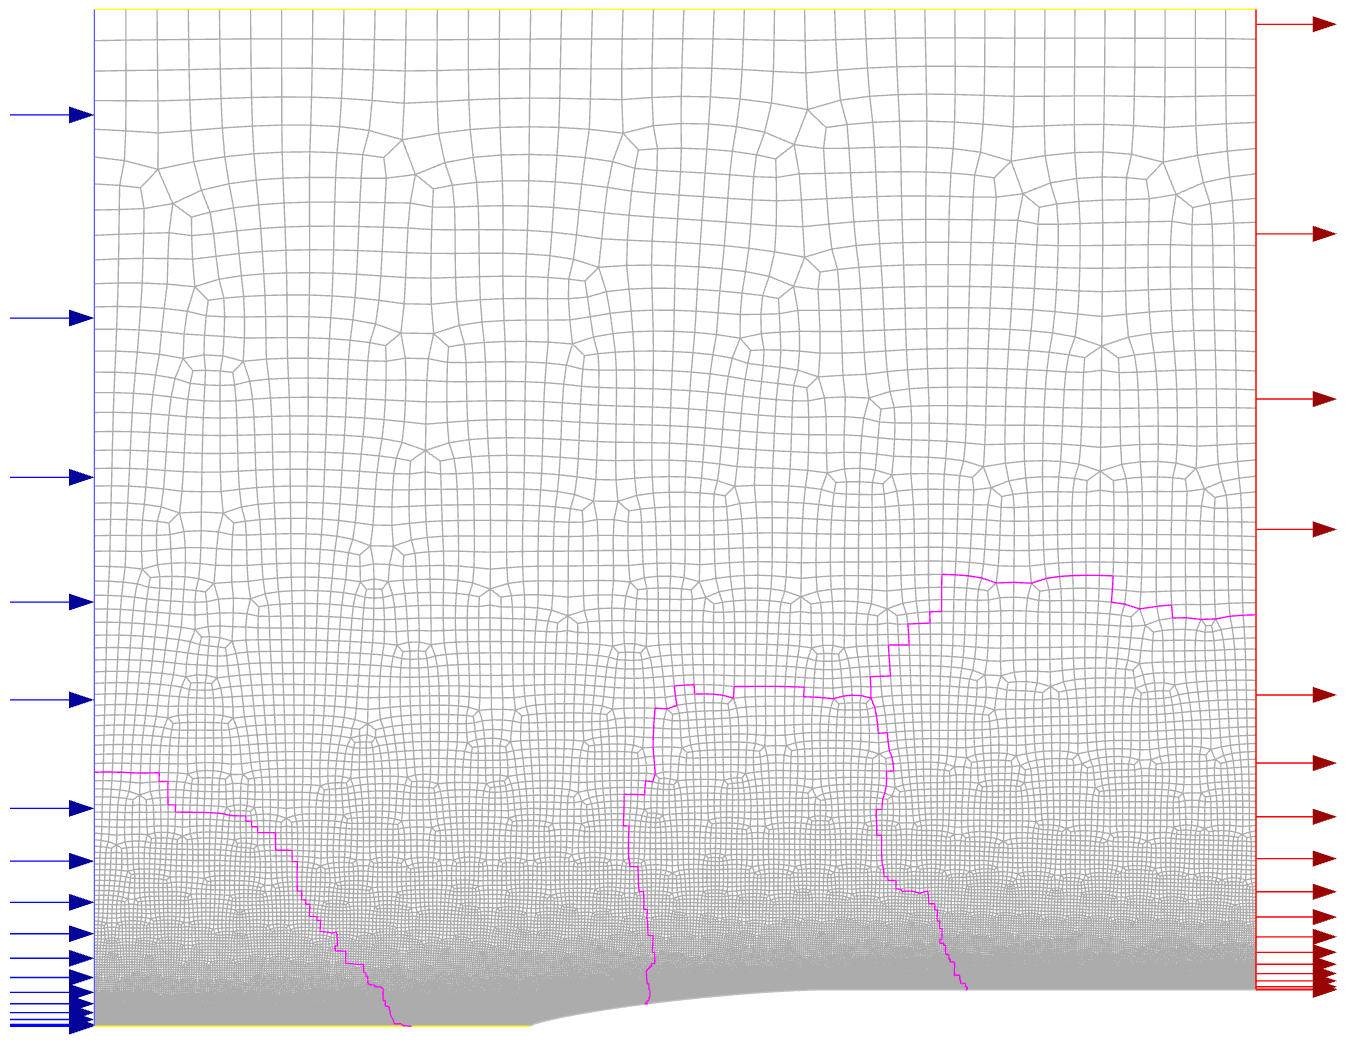
\includegraphics[width=\linewidth]{ansyspost/airflow/mesh_all.png}
  \caption{Darstellung der Außensströmungssimulation mit Meshstruktur in grau, velocity inlet in blau, pressure outlet in rot, Symmetrien in gelb und Partitionen der parallelisierung in lila}\label{fig:aussenstroemung_mesh}
\end{figure}

\begin{figure}[H]
  \centering
  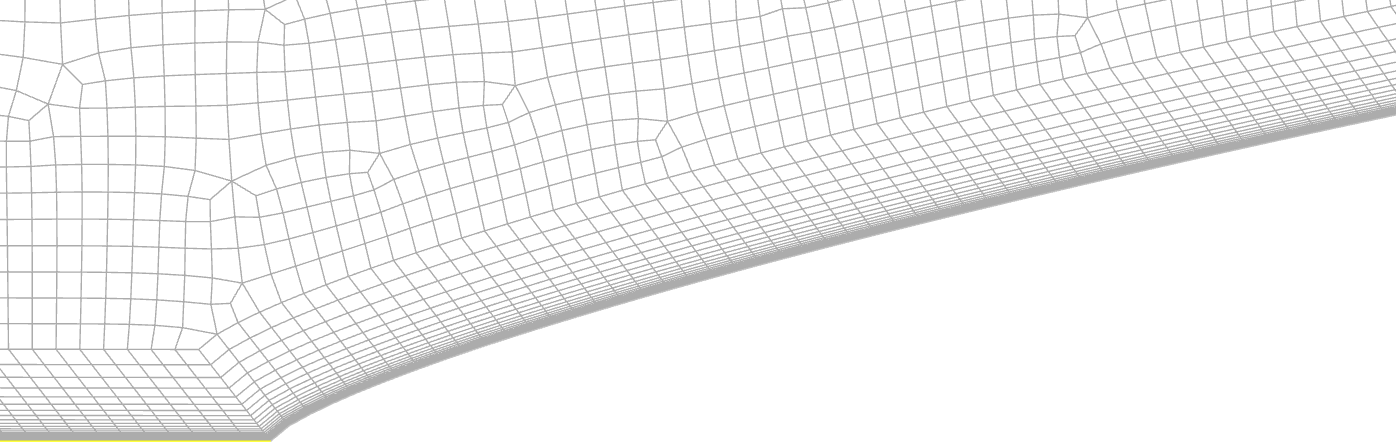
\includegraphics[width=\linewidth]{ansyspost/airflow/mesh_inflation.png}
  \caption{Schichtaufdickungen des Mesh an der Rakete}\label{fig:aussenstroemung_mesh_inflationlayers}
\end{figure}

\begin{figure}[H]
  \centering
  \includegraphics[width=\linewidth]{../../Code/maxQ_compare_heatflux.pdf}
  \caption{Spezifischer Wärmestrom an der Außenhaut bei maximalem dynamischen Druck, sowie \SI{10}{s} davor, danach und \SI{20}{s} danach}\label{fig:spezifischer_waermestrom_maxQ_simulationen}
\end{figure}

\begin{figure}[H]
  \centering
  \includegraphics[width=\linewidth]{../../Code/maxQ_compare_yplus.pdf}
  \caption{y+ Wert an der Außenhaut bei \ac{maxq}, sowie \SI{10}{s} davor, danach und \SI{20}{s} danach}\label{fig:yplus_maxQ_simulationen}
\end{figure}

\begin{figure}[H]
  \centering
  \includegraphics[width=\linewidth]{../../Code/pcm_radiator_hybrid_heatflux_with_sim.pdf}
  \caption{PCM Wärmestrom während Flug mit Simulationsergebnissen und Fit Kurve}\label{fig:pcm_waermestrom_sim}
\end{figure}

\begin{figure}[H]
    \centering

    \begin{subfigure}{\textwidth}
        \centering
        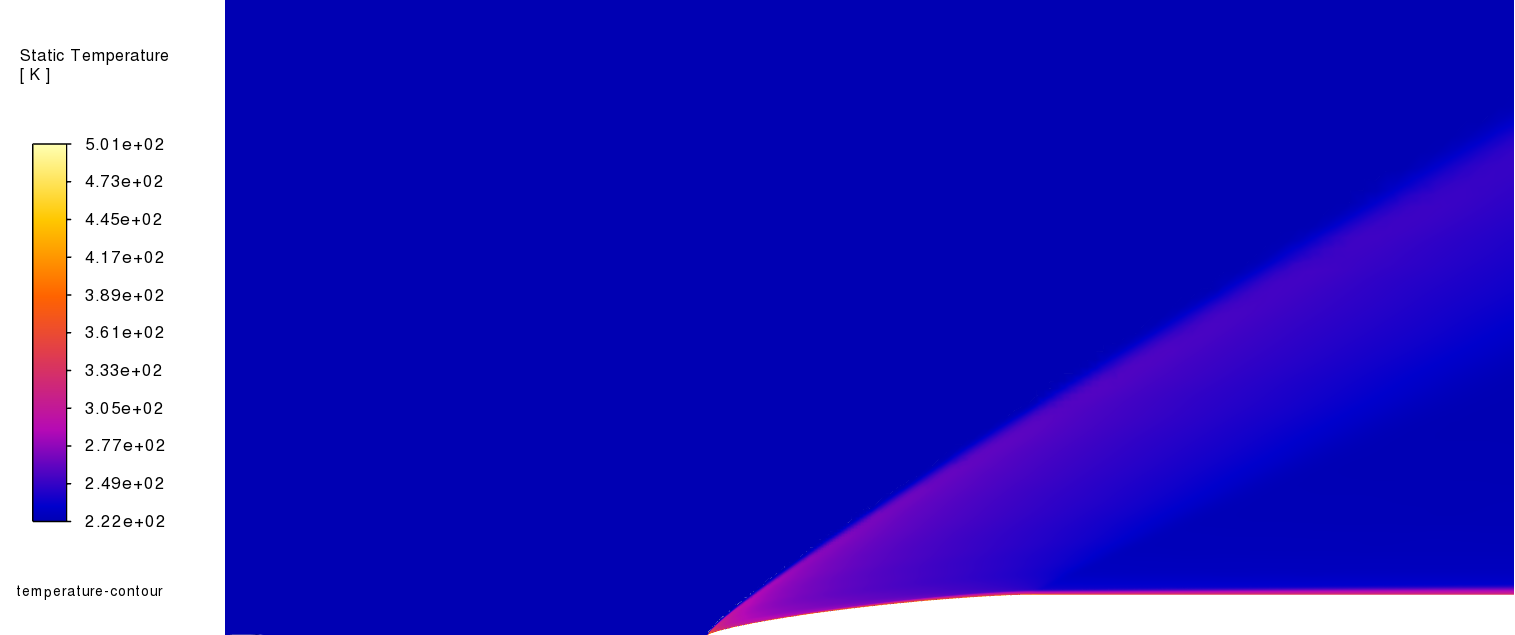
\includegraphics[height=0.23\textheight]{ansyspost/airflow/maxQ-temperature-contour.png}
        \caption{Statische Temperaturkontur der Luft}
        \label{fig:maxQ_temp_contour}
    \end{subfigure}

    \begin{subfigure}{\textwidth}
        \centering
        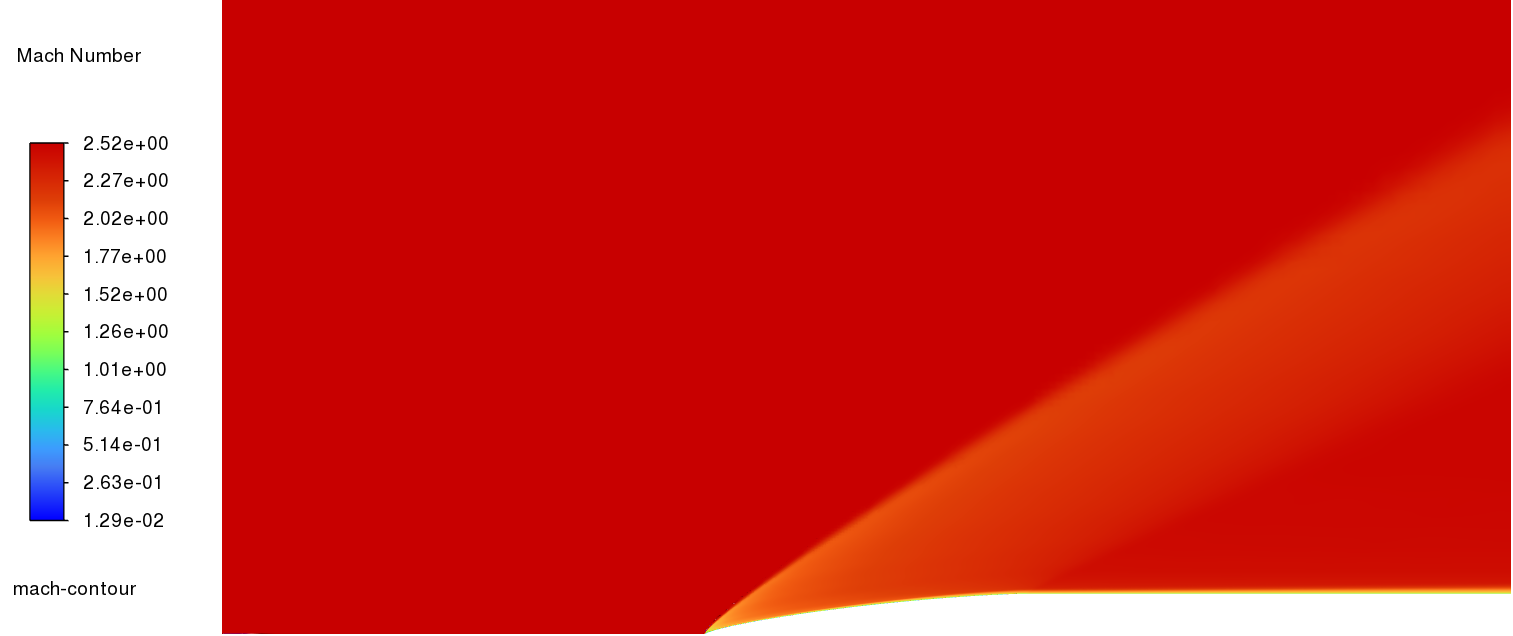
\includegraphics[height=0.23\textheight]{ansyspost/airflow/maxQ-mach-contour.png}
        \caption{Machzahlkontur der Luft}
        \label{fig:maxQ_mach_contour}
    \end{subfigure}

    \caption{\texorpdfstring{\ac{maxq}}{max Q} Konturen der Luft}
    \label{fig:maxQ_konturen}
\end{figure}

\section{PCM}\label{sec:sim_pcm}

Um in ANSYS Fluent Temperaturabhängige Stoffeigenschaften zu implementieren müssen \ac{udf} verwendet werden.
Zu der in \ref{sec:konvektion} behandelten Bossinesq-Approximation \ref{eq:bossinesque} kommen noch 

\begin{figure}[H]
  \centering
  \includegraphics[width=\linewidth]{../../Code/eicosane_cpvst_total.pdf}
  \caption{Effektive spezifische Wärmekapazität von Eicosane}\label{fig:pcm_effective_cp}
\end{figure}

\begin{figure}[H]
  \centering
  \includegraphics[width=\linewidth]{../../Code/eicosane_cpvst_sensible.pdf}
  \caption{Sensible spezifische Wärmekapazität von Eicosane}\label{fig:pcm_sensible_cp}
\end{figure}

\begin{figure}[H]
  \centering
  \includegraphics[width=\linewidth]{../../Code/approximate_acceleration_over_time.pdf}
  \caption{Approximiertes Beschleunigungsprofil}\label{fig:approximierte_beschleunigung}
\end{figure}

\ref{fig:approximierte_beschleunigung} zeigt das Beschleunigungsprofil, welches in der Simulation verwendet wurde. Zu beachten
ist, dass Beschleunigungsspitzen durch den Fallschirm, wie sie in~\ref{fig:acceleration_over_time} gesehen
werden können, ignoriert werden, da diese in einer Überschätzung der Beschleunigung und der Konvektionsvorgänge resultieren würden.


\begin{figure}[H]
    \centering

    % Left figure
    \begin{minipage}[t]{0.485\textwidth}
        \centering
        \setlength{\tabcolsep}{1pt} % reduce subfigure spacing
        % Legend vertically centered & with extra space to right
        \begin{subfigure}[t]{0.16\textwidth}
            \centering
            \raisebox{0.7\height}{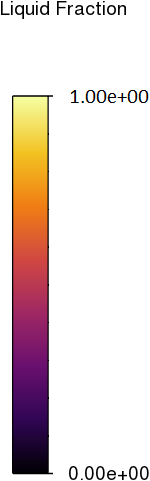
\includegraphics[height=0.2\textheight]{ansyspost/pcm/liquid-fraction-legend.png}}
        \end{subfigure}%
        \hspace{2mm}% extra space between legend and first image
        \begin{subfigure}[t]{0.2\textwidth}
            \centering
            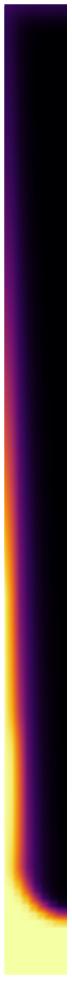
\includegraphics[height=0.5\textheight]{ansyspost/pcm/liquid-fraction-300.png}
            \caption{\SI{300}{\second}}\label{fig:liquid_fraction_300}
        \end{subfigure}%
        \begin{subfigure}[t]{0.2\textwidth}
            \centering
            
\includegraphics[height=0.5\textheight]{ansyspost/pcm/liquid-fraction-600.png}
            \caption{\SI{600}{\second}}\label{fig:liquid_fraction_600}
        \end{subfigure}%
        \begin{subfigure}[t]{0.2\textwidth}
            \centering
            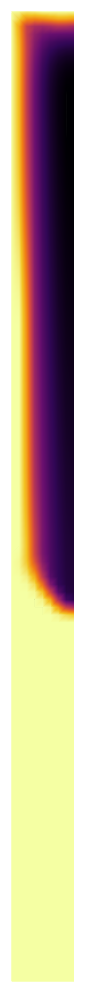
\includegraphics[height=0.5\textheight]{ansyspost/pcm/liquid-fraction-900.png}
            \caption{\SI{900}{\second}}\label{fig:liquid_fraction_900}
        \end{subfigure}%
        \begin{subfigure}[t]{0.2\textwidth}
            \centering
            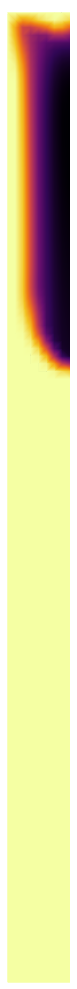
\includegraphics[height=0.5\textheight]{ansyspost/pcm/liquid-fraction-1200.png}
            \caption{\SI{1200}{\second}}\label{fig:liquid_fraction_1200}
        \end{subfigure}
        \caption{Flüssigkeitsanteil Konturen. Die Legende bezieht sich auf~\ref{fig:liquid_fraction_1200}}
        \label{fig:liquid_frac_kontur}
    \end{minipage}
    \hspace{2mm} % small horizontal space
    % Right figure
    \begin{minipage}[t]{0.485\textwidth}
        \centering
        \begin{subfigure}[t]{0.16\textwidth}
            \centering
            \raisebox{0.7\height}{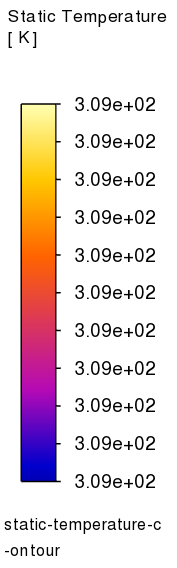
\includegraphics[height=0.2\textheight]{ansyspost/pcm/temperature-legend.png}}
        \end{subfigure}%
        \hspace{2mm}% extra space between legend and first image
        \begin{subfigure}[t]{0.2\textwidth}
            \centering
            
\includegraphics[height=0.5\textheight]{ansyspost/pcm/static-temperature-300.png}
            \caption{\SI{300}{\second}}\label{fig:temperatur_300}
        \end{subfigure}%
        \begin{subfigure}[t]{0.2\textwidth}
            \centering
            
\includegraphics[height=0.5\textheight]{ansyspost/pcm/static-temperature-600.png}
            \caption{\SI{600}{\second}}\label{fig:temperatur_600}
        \end{subfigure}%
        \begin{subfigure}[t]{0.2\textwidth}
            \centering
            
\includegraphics[height=0.5\textheight]{ansyspost/pcm/static-temperature-900.png}
            \caption{\SI{900}{\second}}\label{fig:temperatur_900}
        \end{subfigure}%
        \begin{subfigure}[t]{0.2\textwidth}
            \centering
            
\includegraphics[height=0.5\textheight]{ansyspost/pcm/static-temperature-1200.png}
            \caption{\SI{1200}{\second}}\label{fig:temperatur_1200}
        \end{subfigure}
        \caption{Konturen der statischen Temperatur. Die Legende bezieht sich auf~\ref{fig:temperatur_1200}}
        \label{fig:static_temperature_kontur}
    \end{minipage}

\end{figure}


\begin{lstlisting}[language=C, float, caption={Boussinesq-Approximation des Auftriebs im \ac{pcm} in der \ac{udf} eicosane.c}, label={lst:udf_bossinesque}]
//Y-momentum source
DEFINE_SOURCE(Boussinesq_momentum_source,cell,thread,dS,eqn)
{
	double Temp, source, acc;
	Temp=C_T(cell,thread);

	double t = CURRENT_TIME;

	if (t < 20)
		acc = 34.81;
	else if (t < 50)
		acc = 109.81;
	else if (t < 150)
		acc = 19.62;
	else
		acc = 9.81;

	source=-Rol_pcm*acc*TEC*(Temp-Tr);  //negative for -Y down
	dS[eqn]=-Rol_pcm*acc*TEC; 			//negative for -Y down
	return source;
}
\end{lstlisting}

\begin{figure}[H]
  \centering
  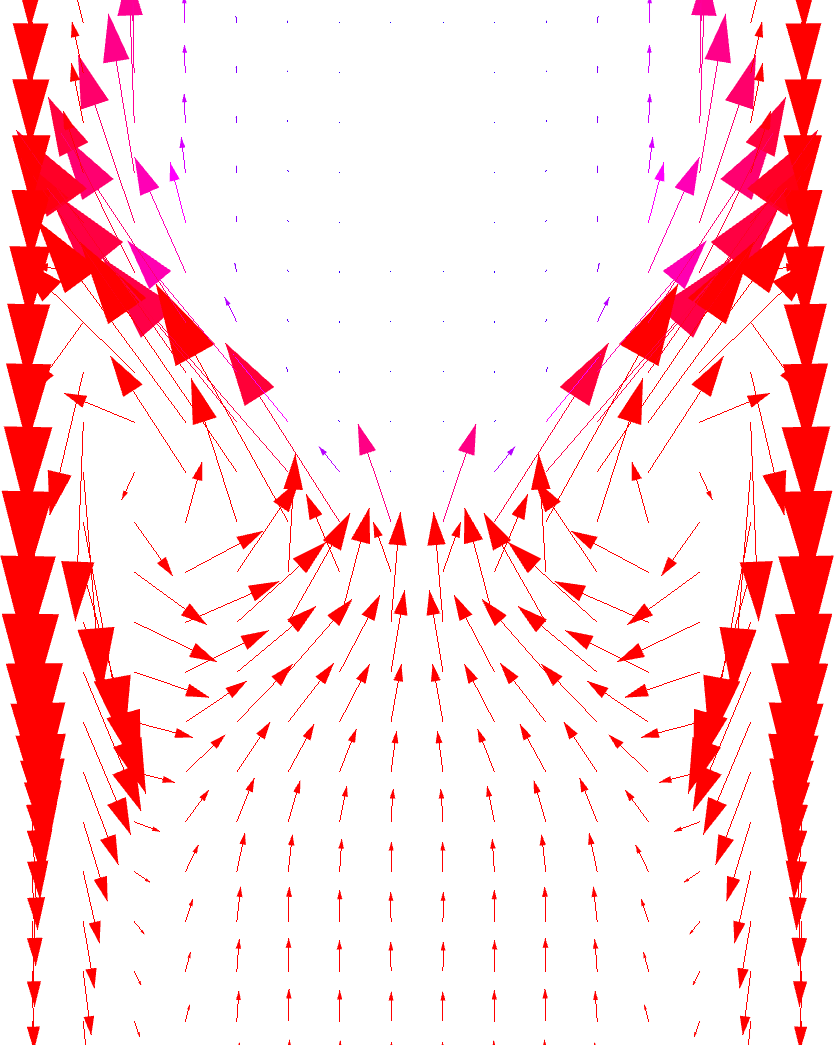
\includegraphics[height=0.4\textheight]{ansyspost/pcm/velocity-vector-close-stitched-900.png}
  \caption{Geschwindigkeitsvektoren der Konvektionswirbel einer, durch Nachbearbeitung, vervollständigten Zelle
  bei \SI{900}{\second}. Darstellung der weiteren Zeitschritte ist in~\ref{fig:pcm_static_temperature_kontur} zu finden.}\label{fig:pcm_vectoren_stitched}
\end{figure}

% ----------- Diskussion & Schlussfolgerungen----------------------------------------
\newpage
\chapter{Discussion and conclusions}
\label{chap:conclusion}
random zeug

Vor der Implementierung des \ac{pcm} in Hardware, sollten die Eigenschaften des vorhandenen n-Eicosan nochmal analysiert und die Ergebnisse überprüft werden.

Wenn man bessere Finnen konstruiert braucht man feineres mesh um gradienten in den wänden zu sehen


Die Vorauslegungwurde mit folgenden Werten durchgeführt:\\
- Isotherm auf: \SI{38}{\celsius}\\
- Avionik Abwärme: \SI{40}{W}\\
- \SI{1}{m} Kontourlänge\\
- Radiator Emissionsgrad: \SI{0,91}{} (AZ-93)\\
- Radiator Absorptionsgrad: \SI{0,15}{} (AZ-93)\\
- Icosane PCM\\
- Trajektoriensimulation\\
- \SI{1}{\kilo\watt\per\meter\squared} mit 50\% dutycycle durch Rotation der Rakete\\
Zu beachten ist, dass die Radiatorleistung konstant bleibt, da das System als isotherm mit einer
infinitesimalen Temperaturerhöhung über den Schmelzpunkt hinweg angenommen wird.\\
Als nächstes sieht man die Flugdaten

\section{Discussion about including pictures}


% ----------- Ausblick --------------------------------------------------------------
\newpage
\chapter{Zusammenfassung und Ausblick}
\label{chap:Ausblick}
\pagestyle{OnlySection}		% wie ganz oben definiert

Beispielliteraturverweise: 

\begin{enumerate}
	\item Fachzeitschrift
	\item Internetquelle
	\item Buch 
	\item Vorlesungsskript
\end{enumerate}

Anmerkung: Es gibt verschiedene Referenzierungsstile 

\subsection{Flüssig-Gas \ac{pcm}}
Eine weitere Methode zum Thermal-Management, die im Rahmen diese Arbeit nicht analysiert wurde, sind Flüsslig-Gas \ac{pcm}'s, welche generell signifikant höhere latente Wärmen haben,
als die hier analysierten Fest-Flüssig Varianten. Beispielsweise hat Ethanol eine Verdampfungsenthalpie von \SI{918000}{J/kg}, also fast das vierfache von Icosane, bei einer
ähnlichen Dichte. Wegen des großen Volumenanstiegs in die Gasphase von Ethanol, ist ein geschlossenes System, welches extremen Drücken standhalten müsste, eher unhandlich. Hierbei würde
das ablassen vom Ethanol in die Atmosphäre die einzige Möglichkeit sein. Da die Rakete jedoch Ethanol als Treibstoff benötigt ist ein betanken der Kühlung vor dem Start keine logistische Schwierigkeit.\\

Signifikante Probleme mit Ethanol als \ac{pcm} wären der relativ hohe Siedepunkt bei \SI{78}{\degreeCelsius}, der entweder durch Druckregelung auf $< \SI{1}{bar}$ in der oberen Atmosphäre
verringert werrden kann, oder das in Kauf nehmen einer heißer laufenden Avionik. Desweiteren verliert das System den großteil der Thermalen Masse, welche bei unvorhergesehenen Verzögerungen
des Fluges und der Recovery die Avionik schneller überhitzen lassen kann als ein geschlossenes System, in dem auch nach dem Phasenwechsel eine hohe Thermale Masse vorhanden ist.

% ----------- Literatur -------------------------------------------------------------
\newpage
\renewcommand{\bibname}{Literaturverzeichnis}

\bibliography{Bibliography/quellen.bib}
\bibliographystyle{plain}%{unsrt}{abbrv}{abbrvnat}{unsrt}

\newpage

%----------- Anhang -----------------------------------------------------------------
\chapter*{Appendix}
\label{chapter:Appendix}
\pagestyle{Appendix}
\addcontentsline{toc}{chapter}{Appendix}

\section*{Appendix A: Vorauslegung}\label{Anh:programmcode}

\begin{figure}[H]
  \centering
  \includegraphics[width=\linewidth]{../../Code/radiator_leistung.pdf}
  \caption{Radiator Leistungskonturen nach Fläche und Temperatur}\label{fig:radiator_flaeche_leistung}
\end{figure}

\begin{figure}[H]
    \centering
    \begin{subfigure}{0.9\textwidth}
        \centering
        \includegraphics[width=\linewidth]{../../Code/pcm_mass.pdf}
        \caption{Konturen der PCM Masse nach Seitenlänge und Höhe der PCM Box}\label{fig:pcm_mass}
    \end{subfigure}
    \vspace{1em}
    \begin{subfigure}{0.9\textwidth}
        \centering
        \includegraphics[width=\linewidth]{../../Code/pcm_heat_capacity.pdf}
        \caption{Konturen der PCM Latent Wärmekapazität nach Seitenlänge und Höhe der PCM Box}\label{fig:pcm_heat}
    \end{subfigure}
    \caption{PCM Auslegung}\label{fig:pcm_mass_heat}
\end{figure}

\newpage

\begin{lstlisting}[language=Python, caption={Funktionen in der hybrid.py}, label={lst:hybrid_python_pseudo}]
    # === flight data ===
    time = raw['time']  # [s]
    velocity = raw['velocity']  # [m/s]
    air_temperature = raw['air_temperature'] + 273.15  # [K]
    acceleration = raw['acceleration']
    air_pressure = raw['air_pressure'] * 100 # [Pa]

    # === constants ===
    eta_0 = 18.27e-6  # [Pa*s]
    T_0 = 291.15      # [K]
    C = 120           # [K]
    kappa = 1.4       # heat capacity ration for air
    R = 287           # [J/(kg*K)]
    c_p = 1005        # [J/(kg*K)]
    x = 1.07          # [m] radiator centerpoint (0.06 m from hull top)
    T_w = 273.15 + target_temperature # [K] PCM melting point

    # === functions ===
    def T_m(T1, T2): return (T1 + T2) / 2                                   # average temperature
    def eta(T): return eta_0 * ((T_0 + C) / (T + C)) * (T / T_0) ** (3/2)   # dynamic viscosity with surherlands formula
    def lam(T): return 2.64638e-3 + 7.326e-5 * T - 1.746e-8 * T**2          # thermal conductivity with polynomial fit
    def rho(p, T): return p / (R * T)                                       # air density
    def Pr(T): return (c_p * eta(T)) / lam(T)                               # prandtl number
    def Ma(V, T): return V / np.sqrt(kappa * R * T)                         # mach number
    def Re(V, p, T, x): return V * rho(p, T) * x / eta(T)                   # reynolds number
    def r(T): return Pr(T) ** (1/3)                                         # recovery factor
    def T_r(V, T): return T * (1 + r(T) * (kappa + 1) / 2 * Ma(V, T))       # recovery temperature
    def qdot_air(p, T, V, x, T_w):                                          # nusselt relation for wall heatflux
        Re_x = Re(V, p, T, x)
        Pr_x = Pr(T)
        Nu_x = 0.0296 * Re_x**0.8 * Pr_x**(1/3) # turbulent
        alpha = Nu_x * lam(T) / x
        return alpha * (T_r(V, T) - T_w)
    def pdyn(V, T, p): return 0.5 * rho(p, T) * V**2                        # dynamic pressure

    # === heatflux calculation ===
    Qdot_env = np.array([
        qdot_air(p, T_m(T_w, T), V, x, T_w)
        for p, T, V in zip(air_pressure, air_temperature, velocity)
    ]) * hybrid_radiator_area + (solar_flux/2 * a * hybrid_radiator_area)  # add solar flux

    Qdot_in = Qdot_env + avionics_power  # [W]

    # === fluid dynamics plot ===
    Re_plot = np.array([Re(V, p, T, x) for V, p, T in zip(velocity, air_pressure, air_temperature)])
    Pr_plot = np.array([Pr(T) for T in air_temperature])
    pdyn_plot = np.array([pdyn(V, T, p) for V, p, T in zip(velocity, air_pressure, air_temperature)])
\end{lstlisting}

\newpage

\begin{lstlisting}[language=C, caption={Vollständige \ac{pcm} \ac{udf} eicosane.c}, label={lst:udf_rest}]
    //Modified UDF of the original source: https://akamcae.com/tutorials/phase-change-material-simulation-in-ansys-fluent/
    #include "udf.h"
    #include "mem.h"

    //n-eicosane constant properties in solid phase
    #define Ros_pcm 910.0
    #define Cps_pcm 2132.4
    #define Ks_pcm 0.4248

    //n-eicosane constant properties in fluid phase
    #define Rol_pcm 769.0
    #define Cpl_pcm 2350.05
    #define Kl_pcm 0.1505

    //thermal expansion coefficient
    #define TEC 0.0009

    //solidus and liquidus temperatures of n-eicosane
    #define Ts 309.0
    #define Tl 311.0

    //reference temperature for Boussinesq's approximation
    #define Tr 310.0		//Fluent Tref must be equal to Tr

    //density of PCM
    DEFINE_PROPERTY(Ro_var_PCM,cell,thread)
    {
        double Gama, Ro_pcm;
        #if !RP_HOST
            Gama=C_LIQF(cell,thread);
            Ro_pcm=(1-Gama)*Ros_pcm+Gama*Rol_pcm;
        #endif
        return Ro_pcm;
    }

    DEFINE_SPECIFIC_HEAT(Cp_var_PCM,T,Tref,h,yi)
    {
        double Gama, Cp_pcm;
        #if !RP_HOST
            if (T<Ts) { Cp_pcm=Cps_pcm; } else if (T>=Ts&&T<=Tl)
            {
                Gama=(T-Ts)/(Tl-Ts);
                Cp_pcm=((1-Gama)*Ros_pcm*Cps_pcm+Gama*Rol_pcm*Cpl_pcm)/((1-Gama)*Ros_pcm+Gama*Rol_pcm);
            }
            else
            {
                Cp_pcm=Cpl_pcm;
            }
            *h=Cp_pcm*(T-Tref);
        #endif
        return Cp_pcm;
    }

    //thermal conductivity of n-eicosane
    DEFINE_PROPERTY(K_var_PCM,cell,thread)
    {
        double Gama, K_pcm;
        #if !RP_HOST
            Gama=C_LIQF(cell,thread);
            K_pcm=(1-Gama)*Ks_pcm+Gama*Kl_pcm;
        #endif
        return K_pcm;
    }

    //dynamic viscosity of PCM with fit
    DEFINE_PROPERTY(Mu_var_PCM,cell,thread)
    {
        double Temp,Mu_pcm;
        #if !RP_HOST
            Temp=C_T(cell,thread);
            Mu_pcm=(9*pow(10.,-4)*pow(Temp,2)-0.6529*Temp+119.94)*pow(10.,-3);
        #endif
        return Mu_pcm;
    }

    DEFINE_SOURCE(Boussinesq_momentum_source,cell,thread,dS,eqn)
    {
        double Temp, source, acc;
        Temp=C_T(cell,thread);

        double t = CURRENT_TIME;

        if (t < 20)
            acc = 34.81;
        else if (t < 50)
            acc = 109.81;
        else if (t < 150)
            acc = 19.62;
        else
            acc = 9.81;

        source=-Rol_pcm*acc*TEC*(Temp-Tr); //negative for -Y down
        dS[eqn]=-Rol_pcm*acc*TEC; //negative for -Y down
        return source;
    }
\end{lstlisting}

% \begin{lstlisting}[language=python, caption={setup.json}, label={lst:setup.json}]
% {
%     "devmode": 0,
%     "avionics_power": 40,
%     "target_temperature": 36.85,
%     "emittance": 0.91,
%     "absorptance": 0.15,
%     "solar_flux": 1000,
%     "trajectory_data_path": "blast.csv"
% }
% \end{lstlisting}

% \begin{lstlisting}[language=python, caption={results.json}, label={lst:results.json}]
% {
%     "hybrid_radiator_area": 0.0996163285294786,
%     "hybrid_radiator_power": 47.471224639710904,
%     "hybrid_capacity_sim": 188087.64535959047,
%     "hybrid_capacity_nu": 626817.5705502237,
%     "pcm_capacity": 48000.0,
%     "hybrid_H_sim": 0.013188203298524867,
%     "hybrid_m_sim": 1.6535028624398134,
%     "hybrid_H_nu": 0.03928567591747304,
%     "hybrid_m_nu": 4.255679378864365,
%     "normal_L_solution": 0.06748627883089094,
%     "normal_m_solution": 0.346609735620966
% }
% \end{lstlisting}

% \begin{lstlisting}[language=python, caption={main.py}, label={lst:main.py}]
% import subprocess

% subprocess.run(["python", "radiator.py"])
% subprocess.run(["python", "hybrid.py"])
% subprocess.run(["python", "pcm.py"])
% subprocess.run(["python", "pcmProperty.py"])
% subprocess.run(["python", "post.py"])
% \end{lstlisting}

% \begin{lstlisting}[language=python, caption={radiator.py}, label={lst:radiator.py}]
% # This Program calculates the steady-state equation for a grey body radiator

% import numpy as np
% import json
% from scipy.constants import Stefan_Boltzmann, pi
% import matplotlib.pyplot as plt
% import matplotlib as mpl



% # === configuration ===
% # load data from setup.json
% try:
%     with open("setup.json", "r", encoding="utf-8") as f:
%         data = json.load(f)
% except FileNotFoundError:
%     print("setup.json not found. Exiting.")
%     exit()
% except json.JSONDecodeError:
%     print("setup.json is empty of invalid. Exiting.")
%     exit()

% DEVELOPMENT_MODE = data["devmode"]
% avionics_power = data["avionics_power"] # W
% e = data["emittance"]
% a = data["absorptance"]
% solar_flux = data["solar_flux"] # W*m^-2
% target_temperature = data["target_temperature"]

% # Set global matplotlib style
% mpl.rcParams.update({
%     "figure.figsize": (4.9, 3.5),
%     "font.size": 11.0,
%     "font.family": "serif",
%     "font.serif": ["cmr10"],
%     "axes.titlesize": "medium",
%     "figure.titlesize": "medium",
%     "text.usetex": not DEVELOPMENT_MODE,
%     "text.latex.preamble": r"\usepackage{amsmath}\usepackage{amssymb}\usepackage[=v2]{siunitx}\usepackage[utf8]{inputenc}"
% })



% # === Equations ===
% rho_alu = 2700 # kg/m^3
% T_target = 273.15+target_temperature # target temperature

% # Define temperature in Celsius for plotting, and convert to Kelvin
% temp_C = np.linspace(0, 100, 100) # ^\circ C
% A = np.linspace(0.01*0.01, 0.3*0.3, 100) # Area [m$^2$]

% A_grid, T_C_grid = np.meshgrid(A, temp_C)
% T_K_grid = T_C_grid + 273.15  # Convert Celsius to Kelvin for calculation

% # Stefan-Boltzmann radiation formula
% phi_radiation = (A_grid * e * Stefan_Boltzmann * T_K_grid**4) # [W]



% # === Target result ===
% hybrid_radiator_area = (avionics_power) / ((e * Stefan_Boltzmann * T_target**4)-(solar_flux/2)*a) # [m^2] necessary radiator area to get rid of avionics- and solarheatflux
% hybrid_radiator_power = hybrid_radiator_area*e*Stefan_Boltzmann*T_target**4 # [W] total out-heatflux of radiator

% # Putting Data into result.json
% with open("result.json", "w", encoding="utf-8") as f:
%     json.dump({}, f, indent=4)  # clear result.json as this is the first write in the programm chain

% data = {
%     "hybrid_radiator_area": hybrid_radiator_area,
%     "hybrid_radiator_power": hybrid_radiator_power
% }

% with open("result.json", "w", encoding="utf-8") as f:
%     json.dump(data, f, indent=4)



% # === Plotting ===
% # Plot
% fig1 = plt.figure(figsize=(8, 6))
% contour = plt.contour(A_grid, T_C_grid, phi_radiation, levels=20, colors='black')
% #plt.colorbar(contour, label='W\"arme [W]')   # colorful contours
% plt.clabel(contour, inline=True, levels=contour.levels[::2], fontsize=10, fmt='%1.1f [W]') # levels makes every second contour have a label
% plt.xlabel(r"Fl\"{a}che [m$^2$]")
% plt.ylabel(r"Temperatur [^\circ C]")
% plt.grid(True)

% if DEVELOPMENT_MODE:
%     plt.title(r"Radiator W\"armestrahlung nach Fl\"{a}che und Temperatur")

% # Save it if not in dev mode
% if not DEVELOPMENT_MODE:
%     fig1.savefig("radiator_leistung.pdf", bbox_inches="tight")

% if DEVELOPMENT_MODE:
%     plt.show()
% \end{lstlisting}

\section*{Appendix B: Simulation}\label{Anh:simulation}

\begin{figure}[H]
    \centering

    \begin{subfigure}{\textwidth}
        \centering
        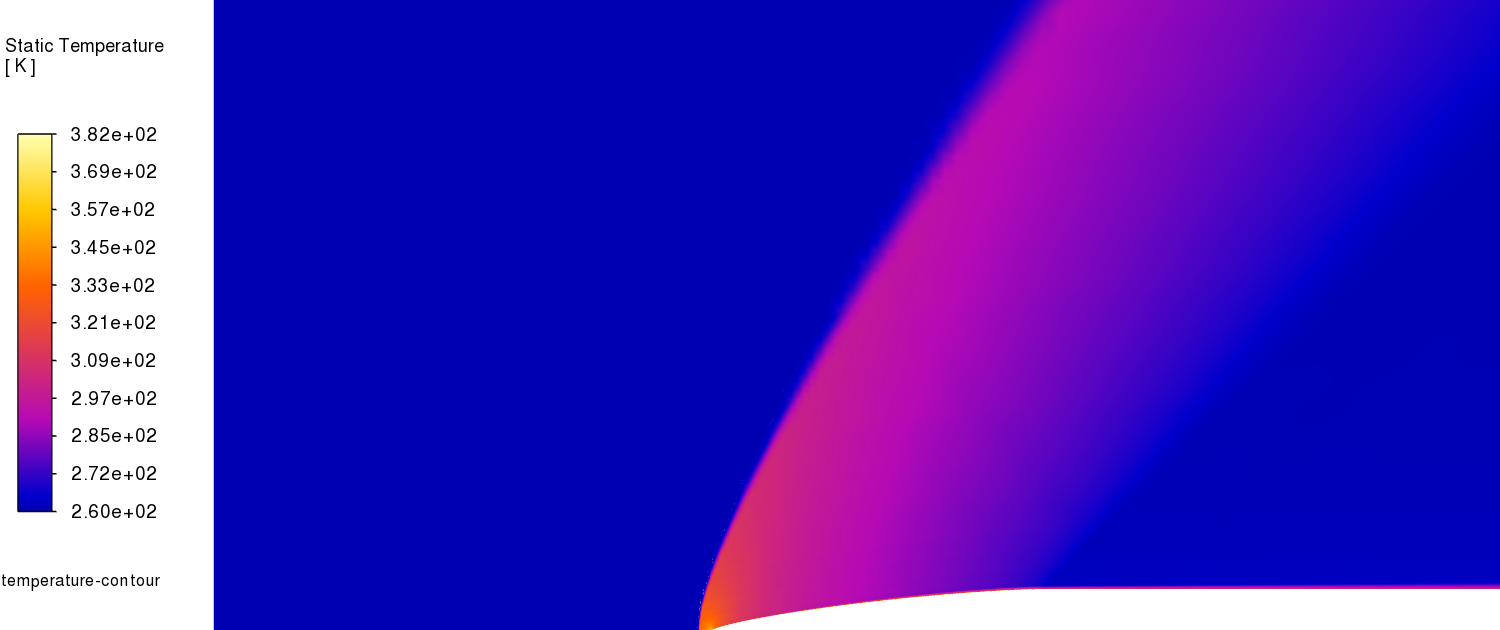
\includegraphics[height=0.23\textheight]{ansyspost/airflow/maxQminus10-temperature-contour.png}
        \caption{\ac{maxq} -\SI{10}{\second}}
        \label{fig:maxQminus10_temp_contour}
    \end{subfigure}

    \begin{subfigure}{\textwidth}
        \centering
        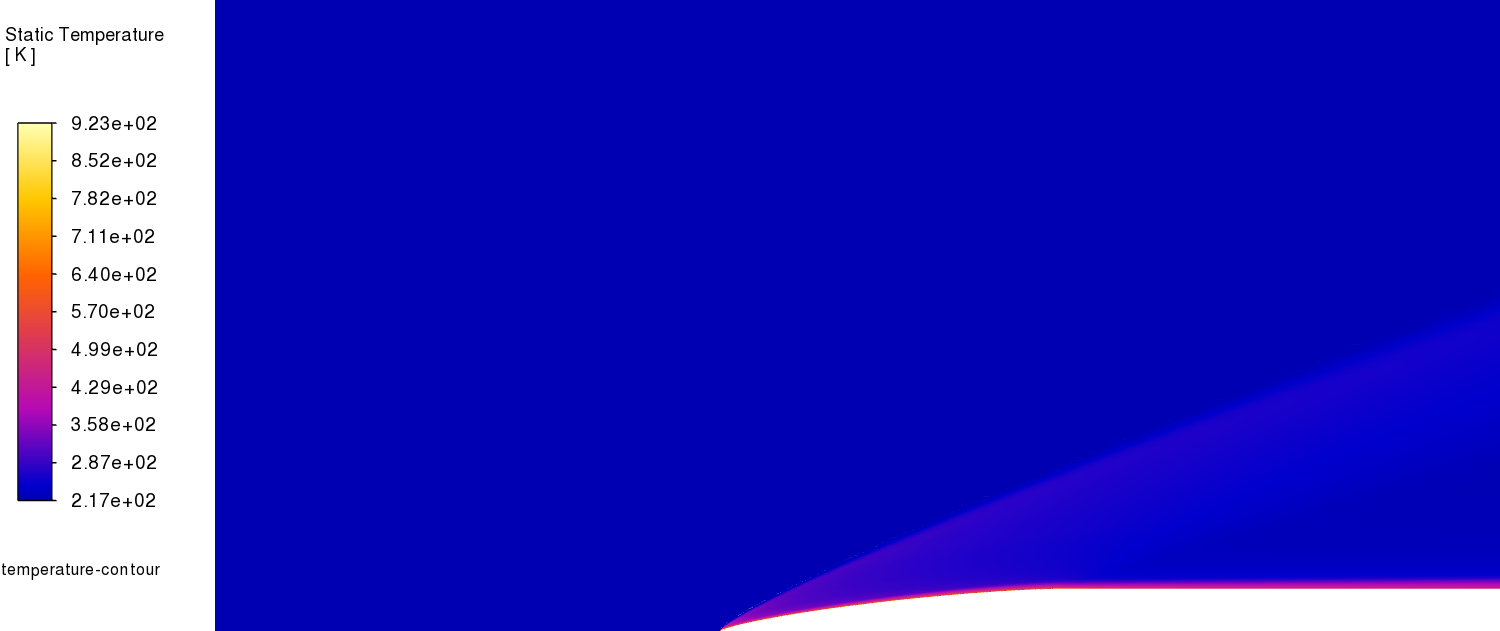
\includegraphics[height=0.23\textheight]{ansyspost/airflow/maxQplus10-temperature-contour.png}
        \caption{\ac{maxq} +\SI{10}{\second}}
        \label{fig:maxQplus10_temp_contour}
    \end{subfigure}

    \begin{subfigure}{\textwidth}
        \centering
        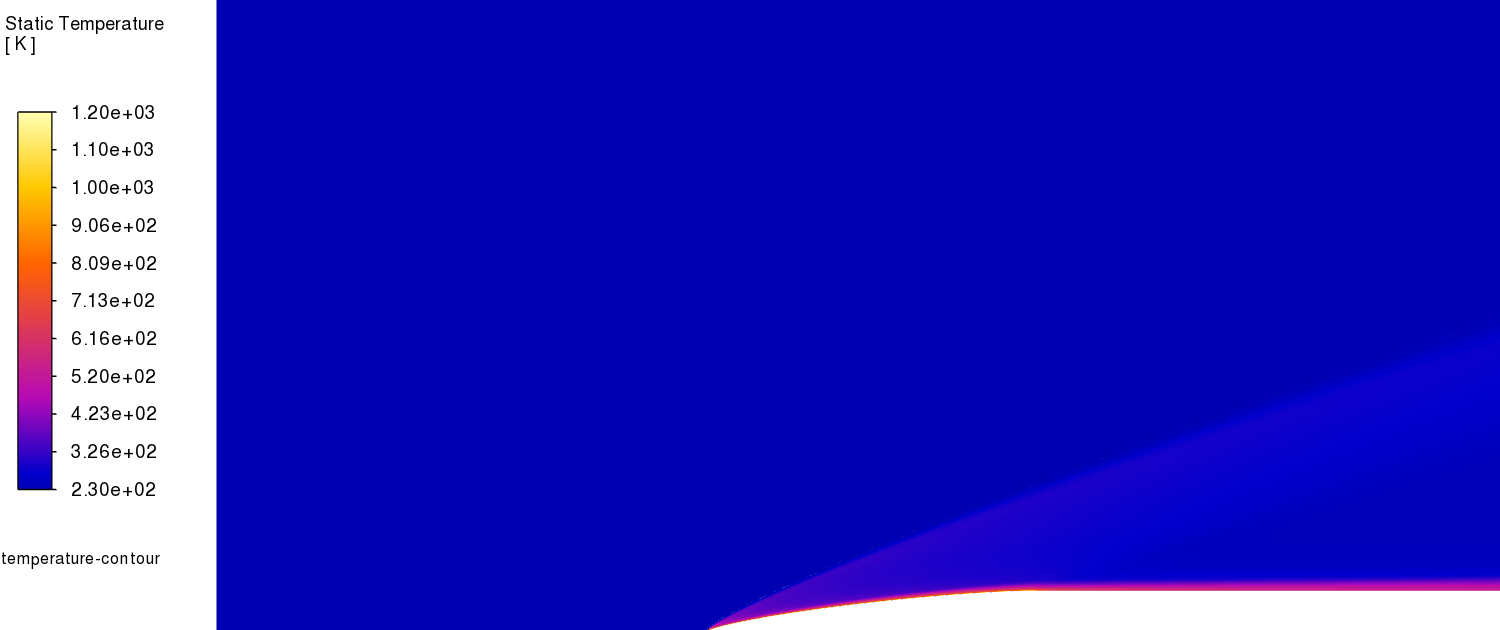
\includegraphics[height=0.23\textheight]{ansyspost/airflow/maxQplus20-temperature-contour.png}
        \caption{\ac{maxq} +\SI{20}{\second}}
        \label{fig:maxQplus20_temp_contour}
    \end{subfigure}

    \caption{Statische Temperaturkontur der Luft}
    \label{fig:airflow_temp_contour_continued}
\end{figure}

\begin{figure}[H]
    \centering

    \begin{subfigure}{\textwidth}
        \centering
        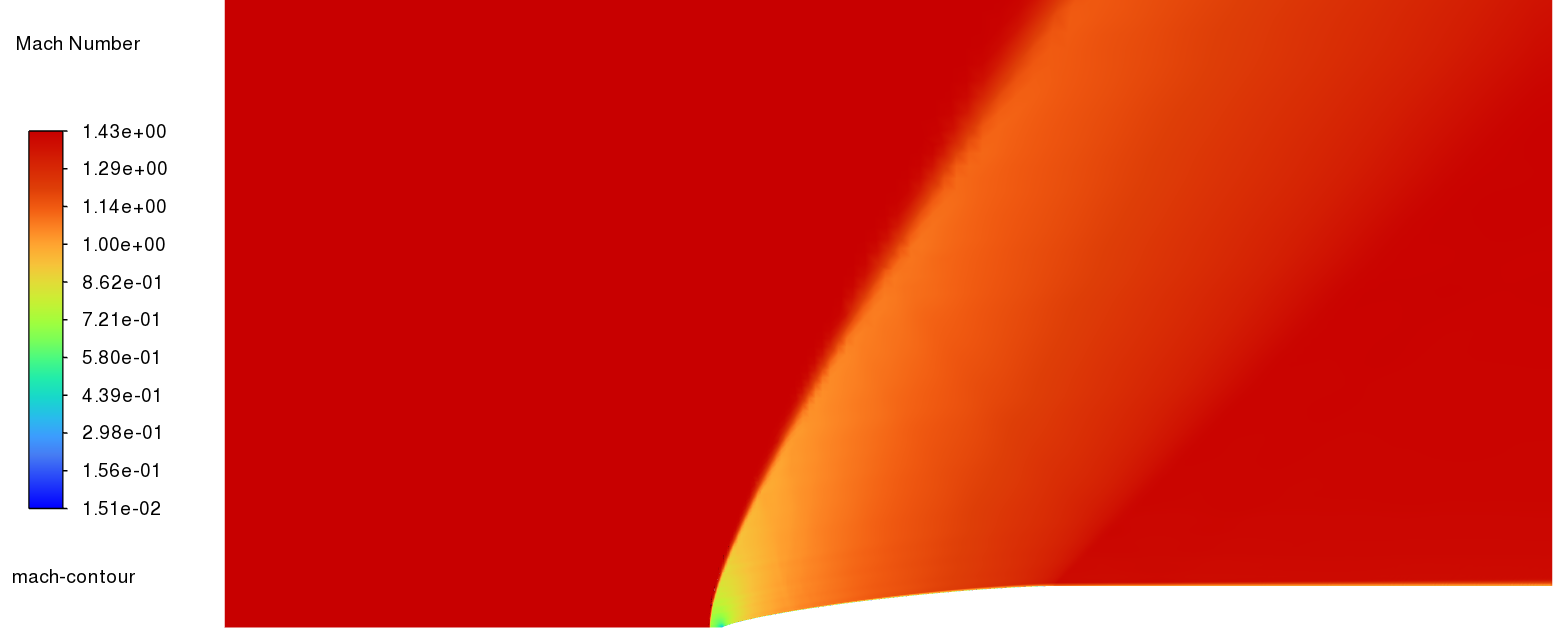
\includegraphics[height=0.23\textheight]{ansyspost/airflow/maxQminus10-mach-contour.png}
        \caption{\ac{maxq} -\SI{10}{\second}}
        \label{fig:maxQminus10_mach_contour}
    \end{subfigure}

    \begin{subfigure}{\textwidth}
        \centering
        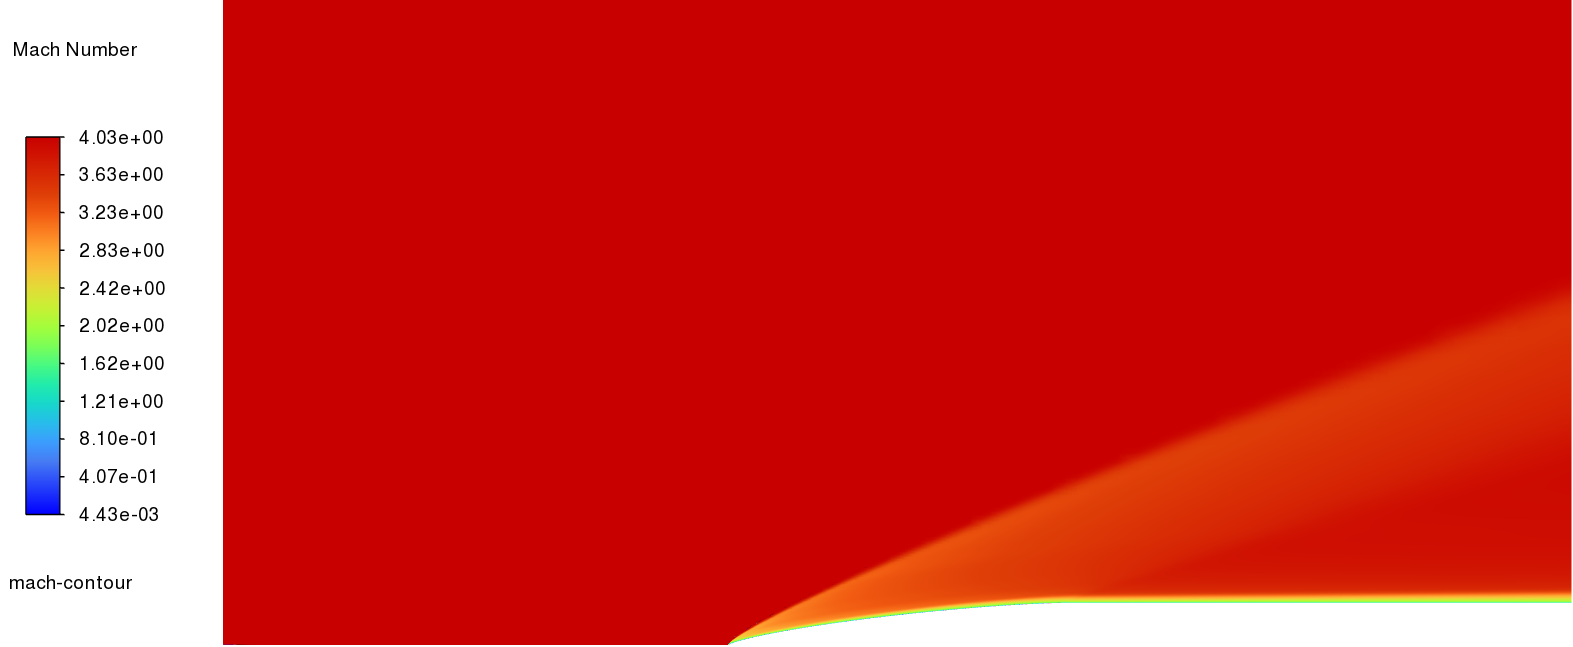
\includegraphics[height=0.23\textheight]{ansyspost/airflow/maxQplus10-mach-contour.png}
        \caption{\ac{maxq} +\SI{10}{\second}}
        \label{fig:maxQplus10_mach_contour}
    \end{subfigure}

    \begin{subfigure}{\textwidth}
        \centering
        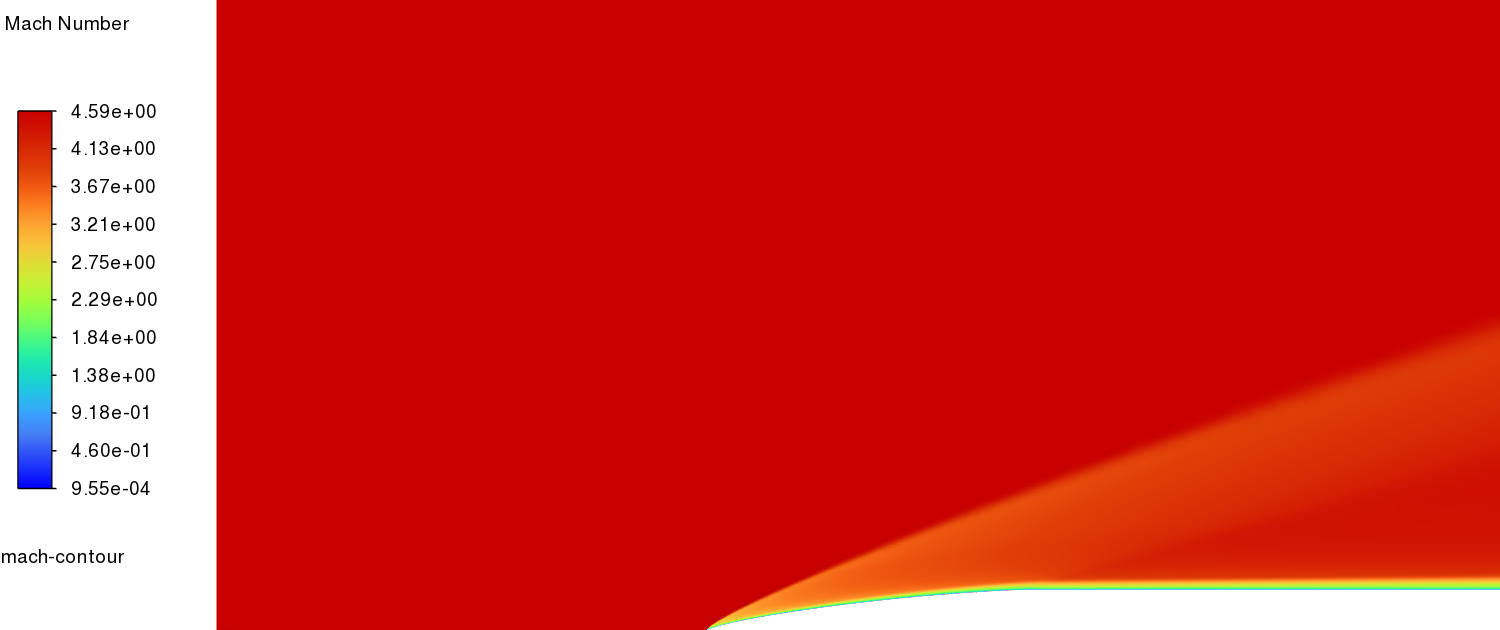
\includegraphics[height=0.23\textheight]{ansyspost/airflow/maxQplus20-mach-contour.png}
        \caption{\ac{maxq} +\SI{20}{\second}}
        \label{fig:maxQplus20_mach_contour}
    \end{subfigure}

    \caption{Machzahlkontur der Luft}
    \label{fig:airflow_mach_contour_continued}
\end{figure}

\begin{figure}[H]
    \centering

    \begin{subfigure}[t]{0.14\textwidth}
        \centering
        \raisebox{1\height}{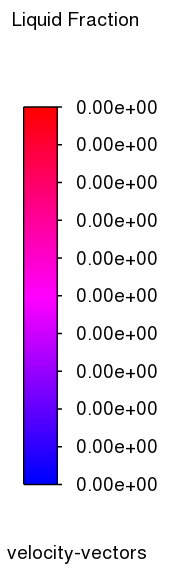
\includegraphics[height=0.2\textheight]{ansyspost/pcm/vector-legend.png}}
    \end{subfigure}%
    \hspace{2mm}% extra space between legend and first image
    \begin{subfigure}[t]{0.2\textwidth}
        \centering
        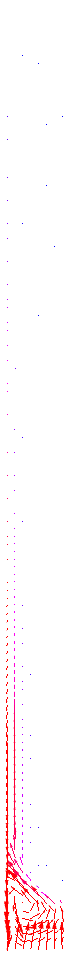
\includegraphics[height=0.7\textheight]{ansyspost/pcm/velocity-vector-300.png}
        \caption{\SI{300}{\second}}\label{fig:velocity_vector_300}
    \end{subfigure}%
    \begin{subfigure}[t]{0.2\textwidth}
        \centering
        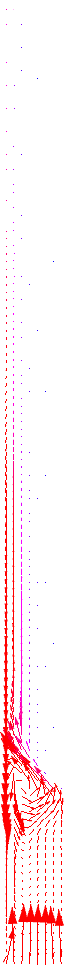
\includegraphics[height=0.7\textheight]{ansyspost/pcm/velocity-vector-600.png}
        \caption{\SI{600}{\second}}\label{fig:velocity_vector_600}
    \end{subfigure}%
    \begin{subfigure}[t]{0.2\textwidth}
        \centering
        \includegraphics[height=0.7\textheight]{ansyspost/pcm/velocity-vector-900.png}
        \caption{\SI{900}{\second}}\label{fig:velocity_vector_900}
    \end{subfigure}%
    \begin{subfigure}[t]{0.2\textwidth}
        \centering
        \includegraphics[height=0.7\textheight]{ansyspost/pcm/velocity-vector-1200.png}
        \caption{\SI{1200}{\second}}\label{fig:velocity_vector_1200}
    \end{subfigure}
    \caption{Konturen der statischen Temperatur. Die Legende bezieht sich auf~\ref{fig:velocity_vector_1200}}\label{fig:pcm_static_temperature_kontur}
\end{figure}

%------------------------------------------------------------------------------------
\end{document}